% Options for packages loaded elsewhere
\PassOptionsToPackage{unicode}{hyperref}
\PassOptionsToPackage{hyphens}{url}
\PassOptionsToPackage{dvipsnames,svgnames,x11names}{xcolor}
%
\documentclass[
  12pt,
]{article}

\usepackage{amsmath,amssymb}
\usepackage{iftex}
\ifPDFTeX
  \usepackage[T1]{fontenc}
  \usepackage[utf8]{inputenc}
  \usepackage{textcomp} % provide euro and other symbols
\else % if luatex or xetex
  \usepackage{unicode-math}
  \defaultfontfeatures{Scale=MatchLowercase}
  \defaultfontfeatures[\rmfamily]{Ligatures=TeX,Scale=1}
\fi
\usepackage{lmodern}
\ifPDFTeX\else  
    % xetex/luatex font selection
\fi
% Use upquote if available, for straight quotes in verbatim environments
\IfFileExists{upquote.sty}{\usepackage{upquote}}{}
\IfFileExists{microtype.sty}{% use microtype if available
  \usepackage[]{microtype}
  \UseMicrotypeSet[protrusion]{basicmath} % disable protrusion for tt fonts
}{}
\makeatletter
\@ifundefined{KOMAClassName}{% if non-KOMA class
  \IfFileExists{parskip.sty}{%
    \usepackage{parskip}
  }{% else
    \setlength{\parindent}{0pt}
    \setlength{\parskip}{6pt plus 2pt minus 1pt}}
}{% if KOMA class
  \KOMAoptions{parskip=half}}
\makeatother
\usepackage{xcolor}
\usepackage[margin=1in]{geometry}
\setlength{\emergencystretch}{3em} % prevent overfull lines
\setcounter{secnumdepth}{5}
% Make \paragraph and \subparagraph free-standing
\makeatletter
\ifx\paragraph\undefined\else
  \let\oldparagraph\paragraph
  \renewcommand{\paragraph}{
    \@ifstar
      \xxxParagraphStar
      \xxxParagraphNoStar
  }
  \newcommand{\xxxParagraphStar}[1]{\oldparagraph*{#1}\mbox{}}
  \newcommand{\xxxParagraphNoStar}[1]{\oldparagraph{#1}\mbox{}}
\fi
\ifx\subparagraph\undefined\else
  \let\oldsubparagraph\subparagraph
  \renewcommand{\subparagraph}{
    \@ifstar
      \xxxSubParagraphStar
      \xxxSubParagraphNoStar
  }
  \newcommand{\xxxSubParagraphStar}[1]{\oldsubparagraph*{#1}\mbox{}}
  \newcommand{\xxxSubParagraphNoStar}[1]{\oldsubparagraph{#1}\mbox{}}
\fi
\makeatother


\providecommand{\tightlist}{%
  \setlength{\itemsep}{0pt}\setlength{\parskip}{0pt}}\usepackage{longtable,booktabs,array}
\usepackage{calc} % for calculating minipage widths
% Correct order of tables after \paragraph or \subparagraph
\usepackage{etoolbox}
\makeatletter
\patchcmd\longtable{\par}{\if@noskipsec\mbox{}\fi\par}{}{}
\makeatother
% Allow footnotes in longtable head/foot
\IfFileExists{footnotehyper.sty}{\usepackage{footnotehyper}}{\usepackage{footnote}}
\makesavenoteenv{longtable}
\usepackage{graphicx}
\makeatletter
\newsavebox\pandoc@box
\newcommand*\pandocbounded[1]{% scales image to fit in text height/width
  \sbox\pandoc@box{#1}%
  \Gscale@div\@tempa{\textheight}{\dimexpr\ht\pandoc@box+\dp\pandoc@box\relax}%
  \Gscale@div\@tempb{\linewidth}{\wd\pandoc@box}%
  \ifdim\@tempb\p@<\@tempa\p@\let\@tempa\@tempb\fi% select the smaller of both
  \ifdim\@tempa\p@<\p@\scalebox{\@tempa}{\usebox\pandoc@box}%
  \else\usebox{\pandoc@box}%
  \fi%
}
% Set default figure placement to htbp
\def\fps@figure{htbp}
\makeatother
% definitions for citeproc citations
\NewDocumentCommand\citeproctext{}{}
\NewDocumentCommand\citeproc{mm}{%
  \begingroup\def\citeproctext{#2}\cite{#1}\endgroup}
\makeatletter
 % allow citations to break across lines
 \let\@cite@ofmt\@firstofone
 % avoid brackets around text for \cite:
 \def\@biblabel#1{}
 \def\@cite#1#2{{#1\if@tempswa , #2\fi}}
\makeatother
\newlength{\cslhangindent}
\setlength{\cslhangindent}{1.5em}
\newlength{\csllabelwidth}
\setlength{\csllabelwidth}{3em}
\newenvironment{CSLReferences}[2] % #1 hanging-indent, #2 entry-spacing
 {\begin{list}{}{%
  \setlength{\itemindent}{0pt}
  \setlength{\leftmargin}{0pt}
  \setlength{\parsep}{0pt}
  % turn on hanging indent if param 1 is 1
  \ifodd #1
   \setlength{\leftmargin}{\cslhangindent}
   \setlength{\itemindent}{-1\cslhangindent}
  \fi
  % set entry spacing
  \setlength{\itemsep}{#2\baselineskip}}}
 {\end{list}}
\usepackage{calc}
\newcommand{\CSLBlock}[1]{\hfill\break\parbox[t]{\linewidth}{\strut\ignorespaces#1\strut}}
\newcommand{\CSLLeftMargin}[1]{\parbox[t]{\csllabelwidth}{\strut#1\strut}}
\newcommand{\CSLRightInline}[1]{\parbox[t]{\linewidth - \csllabelwidth}{\strut#1\strut}}
\newcommand{\CSLIndent}[1]{\hspace{\cslhangindent}#1}

\usepackage{booktabs}
\usepackage{longtable}
\usepackage{array}
\usepackage{multirow}
\usepackage{wrapfig}
\usepackage{float}
\usepackage{colortbl}
\usepackage{pdflscape}
\usepackage{tabu}
\usepackage{threeparttable}
\usepackage{threeparttablex}
\usepackage[normalem]{ulem}
\usepackage{makecell}
\usepackage{xcolor}
\usepackage{setspace}
\usepackage{changepage}
\doublespacing
\usepackage{ragged2e}
\usepackage[table]{xcolor}
\usepackage{float}
\makeatletter
\@ifpackageloaded{caption}{}{\usepackage{caption}}
\AtBeginDocument{%
\ifdefined\contentsname
  \renewcommand*\contentsname{Table of contents}
\else
  \newcommand\contentsname{Table of contents}
\fi
\ifdefined\listfigurename
  \renewcommand*\listfigurename{List of Figures}
\else
  \newcommand\listfigurename{List of Figures}
\fi
\ifdefined\listtablename
  \renewcommand*\listtablename{List of Tables}
\else
  \newcommand\listtablename{List of Tables}
\fi
\ifdefined\figurename
  \renewcommand*\figurename{Figure}
\else
  \newcommand\figurename{Figure}
\fi
\ifdefined\tablename
  \renewcommand*\tablename{Table}
\else
  \newcommand\tablename{Table}
\fi
}
\@ifpackageloaded{float}{}{\usepackage{float}}
\floatstyle{ruled}
\@ifundefined{c@chapter}{\newfloat{codelisting}{h}{lop}}{\newfloat{codelisting}{h}{lop}[chapter]}
\floatname{codelisting}{Listing}
\newcommand*\listoflistings{\listof{codelisting}{List of Listings}}
\makeatother
\makeatletter
\makeatother
\makeatletter
\@ifpackageloaded{caption}{}{\usepackage{caption}}
\@ifpackageloaded{subcaption}{}{\usepackage{subcaption}}
\makeatother

\usepackage{bookmark}

\IfFileExists{xurl.sty}{\usepackage{xurl}}{} % add URL line breaks if available
\urlstyle{same} % disable monospaced font for URLs
\hypersetup{
  colorlinks=true,
  linkcolor={blue},
  filecolor={Maroon},
  citecolor={Blue},
  urlcolor={Blue},
  pdfcreator={LaTeX via pandoc}}


\author{}
\date{}

\begin{document}


\begin{titlepage}
  \centering
  
\includegraphics[width=1\textwidth]{images/hertie-school-logo.jpg}
  \vspace*{\fill}
  
  \textbf{Enabling Jurimetrics: Deploying Open‑Source Large Language Models for Empirical Insights into Brazilian Courts}\\

  \vspace{2.5cm}

  Rodrigo Filippi Dornelles

  \vspace{1cm}
  
  Master of Data Science for Public Policy, Class of 2025\\
  
  \vspace{0.5cm}

  Berlin, April 28, 2025\\

  \vspace*{\fill}

  Supervised by Prof. Lynn Kaack, PhD
  \vspace{0.5cm}
  
  Word count: 7,642 words
\end{titlepage}

\section[Executive Summary]{\texorpdfstring{Executive
Summary\footnote{The GitHub repositiry of this research is available at:
  \url{https://github.com/rfdornelles/hertie_mds_master_thesis}}}{Executive Summary}}\label{sec-executive-summary}

Empirical analyses of court decisions---jurimetrics---remain rare in
Brazil. Recent advances in open-source large language models (LLMs)
create an opportunity to automate the extraction of structured data from
these decisions at a fraction of the cost of proprietary systems while
preserving privacy and reproducibility. This thesis asks whether
open-source LLMs can match or surpass leading commercial models when
deployed end-to-end on Brazilian judicial cases.

A gold-standard corpus of 258 São Paulo drug-trafficking sentences
(\citeproc{ref-lacerda_e_silva_punindo_2021}{Lacerda e Silva, 2021}) was
split into training, validation, and test sets. Twelve base
models---seven open-source, five commercial---were benchmarked
zero-shot.The best open-source model (Gemma 3-27B) already outperformed
GPT-4o, achieving 0.82 accuracy versus 0.79 on 39 held-out cases. Three
models (GPT-4o-mini, Phi-4 14B, and Llama-3 3B) were fine-tuned via LoRA
and quantization. Fine-tuning raised Phi-4's accuracy to 0.92,
statistically indistinguishable from the commercial leader yet 25 \%
cheaper and twice as energy-efficient when labeling a new batch of 454
cases. Llama-3 3B, with one-fifth the parameters of Phi-4, reached 0.78
of accuracy at less than half the cost and inference time, illustrating
an attractive speed-versus-quality trade-off for large-scale annotation.

These findings confirm the ``power of specialization''
(\citeproc{ref-dominguez-olmedo_lawma_2024}{Dominguez-Olmedo et al.,
2024}): modest amounts of high-quality domain data can lift open-source
LLMs to state-of-the-art performance in legal information extraction.
The work contributes to an end-to-end pipeline, open-source code and
evaluation scripts, and practical guidance on model selection,
fine-tuning, and deployment under tight resource constraints. It
demonstrates a feasible, transparent, and affordable path toward
large-scale, data-driven legal research in civil law jurisdictions. It
also supports policy calls for greater data openness, interdisciplinary
training, and investment in public-interest NLP infrastructure.

\newpage{}

\tableofcontents
\newpage
\listoffigures
\newpage
\listoftables
\thispagestyle{empty}
\newpage
\thispagestyle{empty}
\vspace*{\fill}
\begin{flushright}
\begin{minipage}{0.45\textwidth}
\singlespacing
\justifying
\textit{\fontsize{10}{12}\selectfont
"In the end, the way we use [artificial intelligence] to include the least of our brothers and sisters, the vulnerable and those most in need, will be the true measure of our humanity."
}

\vspace{1ex}
\begin{flushright}
\textit{Pope Francis\footnotemark}
\end{flushright}
\end{minipage}
\end{flushright}

\footnotetext{Message for the LVII World Day of Peace, 1 January 2024.}
\vspace*{0pt}
\newpage

\section{Introduction}\label{sec-introduction}

\vspace*{\fill}
\noindent\hfill
\begin{minipage}{0.50\textwidth}
\singlespacing
\justifying
\textit{\fontsize{10}{12}\selectfont"I promise to practice Law with dignity and independence, to observe ethics, professional duties and prerogatives and to defend the Constitution, the legal order of the Democratic State, human rights, social justice, the proper application of laws, the rapid administration of justice and \textbf{the improvement of legal culture and institutions}."
}
\vspace{1ex}
\begin{flushright}
\textit{Oath of the Legal Profession\footnotemark}
\end{flushright}
\end{minipage}

\footnotetext{\mbox{Art.} 20, General Regulation of the Statute of the Lawyer Professorship, Brazilian Bar Association}
\vspace*{\fill}

Law, in every modern democracy, is more than a set of abstract norms; it
is a living institutional mechanism through which policy choices are
translated into concrete incentives, constraints, and remedies. To
evaluate whether a legal system fulfills that role, we must ask not only
\textbf{what} the statutes prescribe but \textbf{how} they are applied:
How long does a civil action typically last? What compensation do
consumers actually receive? Which factors shape sentencing in
drug-trafficking cases? These eminently empirical questions are still
surprisingly difficult to answer.

More than half a century ago, Lee Loevinger
(\citeproc{ref-loevinger_jurimetricsnext_1948}{1948}) coined the term
\emph{jurimetrics} to describe the systematic, quantitative study of
law. While the movement gained traction in the United States, it has
remained underutilized in civil-law jurisdictions like Brazil. Recent
initiatives---for example, the Associação Brasileira de
Jurimetria\footnote{\url{https://abj.org.br/}} and the Rede de Estudos
Empíricos em Direito\footnote{\url{https://reedpesquisa.org/}}---have
begun to fill the gap, yet the volume and heterogeneity of judicial
documents continue to deter large-scale analysis.

The arrival of large language models (LLMs) changes that calculus. Since
the public debut of GPT-3.5 and ChatGPT, the natural language processing
community has released a stream of increasingly capable---and
increasingly efficient---models. Crucially, many cutting-edge
architectures are now open-source: Llama-3, Gemma-3, Phi-4, and kindred
efforts come with permissive licenses that suit academic and
public-sector deployment. Coupled with parameter-efficient fine-tuning
techniques and low-bit quantization, these models can, in principle,
extract structured data from thousands of judgments on commodity
hardware.

This thesis explores whether that promise holds for Brazilian courts. It
pursues three objectives. First, it benchmarks leading commercial LLMs
on information extraction from complex judicial sentences, establishing
a performance and cost baseline. Second, it evaluates a portfolio of
open-source models, addressing practical hurdles such as limited context
windows and the absence of native JSON output. Third, it fine-tunes the
most promising open-source candidates on a modest, expert-annotated
corpus to test the ``power of specialization'' hypothesis advanced by
Dominguez-Olmedo et al.
(\citeproc{ref-dominguez-olmedo_lawma_2024}{2024}). The comparative
results are analyzed regarding accuracy, inference time, energy
consumption, and monetary cost, yielding evidence-based recommendations
for researchers, courts, and policy-makers.

By demonstrating a reproducible, affordable pipeline for large-scale
jurimetric studies, the project aims to move empirical legal research in
Brazil from the margins to the mainstream---and, in doing so, to
strengthen the evidentiary foundations of public policy.

\section{Related Work}\label{related-work}

\subsection{Teorethical Framework}\label{sec-teorethical-framework}

This research relies on data science
(\citeproc{ref-wickham_r_2023}{Wickham et al., 2023}) applied to natural
language processing tasks (\citeproc{ref-vajjala_practical_2020}{Vajjala
et al., 2020}), specifically large language models
(\citeproc{ref-raschka_build_2024}{Raschka, 2024}) powered by recent
advancements in the field due to deep learning techniques
(\citeproc{ref-zhang_dive_2023}{Zhang et al., 2023}).

\subsection{Empirical Legal Research}\label{empirical-legal-research}

The field of empirical research should be intended as a method of
studying law in which we shift the focus from the normative aspect of
law to `its concrete manifestation'
(\citeproc{ref-alves_da_silva_aspectos_2022}{Alves da Silva, 2022}).

As a materialization of this, there were outstanding examples of
high-quality data-driven legal research: Costa et al.
(\citeproc{ref-costa_eficacia_2011}{2011}) studied a comprehensive
amount of judicial decisions regarding administrative misconduct,
concluding the efficiency of the existing legislation. Associação
Brasileira de Jurimetria
(\citeproc{ref-associacao_brasileira_de_jurimetria_avaliacao_2019}{2019})
contributed to the criminal law field, describing how judicial decisions
evaluate the line between a drug user and a drug dealer according to the
amount of drug seized.

Still, in drug possession cases, Lacerda e Silva
(\citeproc{ref-lacerda_e_silva_punindo_2021}{2021}) dived into judicial
sentences to identify the effect of gender and race biases in the
decisions, in which older Black men often receive harsher sentences.
Lately, Instituto de Pesquisa Econômica Aplicada (Ipea) \& Brasil.
Ministério da Justiça e Segurança Pública
(\citeproc{ref-instituto_de_pesquisa_economica_aplicada_ipea_perfil_2023}{2023})
has provided the most comprehensive research in the field, analyzing a
few thousand judicial cases in depth and giving important insights about
how drug legislation is being applied in the whole country.

Although those gold-standards studies, Cabrera De Bonito et al.
(\citeproc{ref-cabrera_de_bonito_pesquisa_2025}{2025}) recently mapped
the landscape of empirical legal research in Brazil, pointing out that
despite relevant developments in the field, quoting Dragoni et al.
(\citeproc{ref-dragoni_combining_2016}{2016}), `the results remain
unsatisfactory.'

Jurimetrics (\citeproc{ref-loevinger_jurimetricsnext_1948}{Loevinger,
1948}) is also, according to Cabrera De Bonito et al.
(\citeproc{ref-cabrera_de_bonito_pesquisa_2025}{2025}), an attempt to
bring empirical methods to law. However, it remains ``little explored in
countries with a Roman-Germanic legal tradition, such as Brazil,''
largely due to methodological gaps from practitioners (Andrade
(\citeproc{ref-de_andrade_utilizacao_2018}{2018}) quoted by Cabrera De
Bonito et al. (\citeproc{ref-cabrera_de_bonito_pesquisa_2025}{2025})).

Ribeiro et al. (\citeproc{ref-ribeiro_jurimetria_2022}{2022}) pointed to
a rise in the field of jurimetrics in Portuguese, although it remains
little compared to the USA. In a search in Google Scholar (12. set.
2021), they identify that the Portuguese translation\footnote{Important
  to mention that in Spanish, the translation would be spelled in the
  same way} `jurimetria' is found in 814 results, although `jurimetrics'
results 16.600. Replicating the search (18.04.2025), we have found 2.270
versus 21.800, meaning that the proportion has considerably increased
while there is still a relevant gap.

Also, Ribeiro et al. (\citeproc{ref-ribeiro_jurimetria_2022}{2022})
identified an important challenge to the practice of jurimetrics: the
lack of uniformity in Legal documents. That is why it makes sense to try
LLMs, as they strive for this task due to their flexibility in context
understanding.

Representing a more recent study of legal implications, Benatti et al.
(\citeproc{ref-benatti_gender_2024}{2024}) shed light on gender
inequalities in the legal discourse by applying NLP methods and pointed
out the importance of having good-quality data in a reasonable amount.

The lack of high-quality models in Portuguese might pose a challenge. In
this sense, the work of Niklaus et al.
(\citeproc{ref-niklaus_multilegalpile_2023}{2023}), Almeida et al.
(\citeproc{ref-almeida_sabia-2_2024}{2024}), and Pires et al.
(\citeproc{ref-pires_sabia_2023}{2023}) in building good-quality models
in this language pointed out a good path to our research.

Lastly, the papers from Dominguez-Olmedo et al.
(\citeproc{ref-dominguez-olmedo_lawma_2024}{2024}) and Junior et al.
(\citeproc{ref-junior_juru_2024}{2024}) were especially relevant to our
work. The first didactically showed the lack of annotations as a
`bottleneck for the field of empirical legal studies' and suggested a
strategy that we adopt here: ``Obtain a few hundred labeled examples,
fine-tune an open source model, and use the fine-tuned model to annotate
the remaining cases''
(\citeproc{ref-dominguez-olmedo_lawma_2024}{Dominguez-Olmedo et al.,
2024}).

Junior et al. (\citeproc{ref-junior_juru_2024}{2024}) also identified
the potential of ``domain specialization'' when they fine-tuned a model
using domain data, achieving improvements in efficiency and accuracy at
the cost of degradation of performance in general-knowledge tasks. It
should be a fair price to pay in the context of this work.

\subsection{The research gap}\label{the-research-gap}

Although there are good examples of high-quality empirical data, there
is still little work to be done to apply LLMs in Portuguese \textbf{and}
legal. Another challenge is using little data and, preferably,
open-source models since they are more suitable for academic and
public-sector settings.

On the one hand, we recognize a research gap regarding the lack of
empirical legal research, mainly in Brazil. On the other hand, we see an
opportunity to apply the findings of the fast-paced field of natural
language processing empowered by modern deep learning techniques.

\section{Research Question}\label{sec-research_question}

Can open-source large language models be deployed in the Brazilian legal
context to accurately extract information, recognize entities, and draw
conclusions from complex legal documents, compared to leading
proprietary systems?

\section{Data Sources and Models}\label{sec-data_sources_models}

\subsection{Datasets}\label{sec-datasets}

Given the goals of this research, it would be necessary to gather a
dataset containing judicial decisions and annotations over the features
of interest. Theoretically, this deep learning method could be applied
to any setting of judicial decisions as long as enough data and labels
were available to represent the chosen features. The better the amount
and quality of the data, the better the performance of the models over
it.

The primary data needed for this research is a comprehensive amount of
judicial decisions. Given the Brazilian Judiciary branch's
digitalization, scrapping this data from the source is not a huge
technical challenge. However, obtaining labels and annotations in
addition to the raw text of judicial decisions was fundamental. In
testing and fine-tuning models, we should have a set of decisions and
the features already extracted from them.

Given the scope of this research and the need for at least a few hundred
observations, the manual label was not feasible. So, instead of doing
manual work to build a new dataset, the decision was to try to obtain
data from other legal empirical researchers, such as Costa et al.
(\citeproc{ref-costa_eficacia_2011}{2011}), which was not available.

Also, we have tried to access Instituto de Pesquisa Econômica Aplicada
(Ipea) \& Brasil. Ministério da Justiça e Segurança Pública
(\citeproc{ref-instituto_de_pesquisa_economica_aplicada_ipea_perfil_2023}{2023})
microdata to build a golden dataset since they have about 3.5k data
points labeled through a filing a freedom of information request. It
would have been a unique asset since the data was comprehensive
regarding virtually all Common Justice Courts in Brazil, and, given the
large size, it would be possible to try different training datasets and
have a more comprehensive test dataset.

Due this request, is now possible to access the
\href{https://www.gov.br/mj/pt-br/assuntos/sua-protecao/politicas-sobre-drogas/pesquisa-e-informacao-3/pesquisa\%20IPEA/pesquisa-ipea-perfil-processado-e-producao-de-provas}{general
dataset}. Nevertheless, despite many attempts to convince the provider,
they have not provided the lawsuit identifier, so it was not possible to
match each row in their dataset to a legal case and, therefore, to a
specific document.

\subsubsection{Lacerda's Dataset}\label{lacerdas-dataset}

Lacerda e Silva (\citeproc{ref-lacerda_e_silva_punindo_2021}{2021})
collected in her master's thesist cases from the São Paulo State Court
of Justice (TJSP), focusing on a sample covering 2017 and 2018.
Approximately 35 features were manually annotated and labeled for each
case. In this research, despite focusing only on São Paulo's Court of
Justice (which is, by its turn, the biggest Court in Latin America),
annotations were made in about 400 legal cases related to drug
trafficking. Access to the dataset was obtained by contacting the
researcher, who provided it for further adaptation to this research.

Some of the original features also referred to other documents rather
than the judicial decision, and, therefore, they were excluded (since it
would not be reasonable that the model inferred that). Features related
to biological data were also excluded for ethical reasons.

The documents used initially for each decision case analyzed by the
Lacerda Dataset were extracted automatically from the TJSP database. We
decided to re-collect data since, besides relevant parts of the original
documents being only available in PDF, they also contained pieces of the
political investigation collected from primary sources and were not
available to the public. Also, this choice was relevant to respect
privacy and be closer to real-life settings, where the data would likely
come from the Court's public website.

Since no official API exists to collect data, the process used the Filho
\& Trecenti (\citeproc{ref-filho_coleta_2020}{2020}) R package called
\{tjsp\}. It gathered metadata of each case and the judicial decision
text in string format in an R data frame. In some circumstances, when
the respective decision was not available on the public consultation
website, it was manually re-collected in PDF format and read
automatically using R\footnote{Through the package pdftools}.

After transformation and data wrangling\footnote{Mainly using the
  packages dplyr and tidyr in R}, the final dataset contained 50 columns
to adapt the data to this research. The different number of columns was
due to some categorical features being transformed into boolean so that
the model could extract it easier and less likely to lose information.
For instance, the column \emph{DenDrogas} contained information about
the most common articles of Law in the accusation. It was transformed
into the columns \emph{denuncia\_art\_33}, \emph{denuncia\_art\_34}, and
\emph{denuncia\_art\_35}.

In addition, some duplicates and redundancies were excluded, and some
documents were not collected due to missingness in the original dataset;
the final result was a dataset with 258 cases, which were split into
training (186 cases), test (39 cases), and validation (33 cases).

Finally, we decided to store the data in the .parquet format. This
choice preserved the original column types and allowed seamless data
interchange between Python and R.

\subsection{Models}\label{sec-models}

In choosing the models, we tried to blend those that are specific to use
cases (\citeproc{ref-dominguez-olmedo_lawma_2024}{Dominguez-Olmedo et
al., 2024}), in Portuguese (\citeproc{ref-correa_tucano_2024}{Corrêa et
al., 2024}; \citeproc{ref-pires_sabia_2023}{Pires et al., 2023}), or
representative of the state-of-the-art
(\citeproc{ref-abdin_phi-4_2024}{Abdin et al., 2024};
\citeproc{ref-openai_gpt-4_2024}{OpenAI et al., 2024};
\citeproc{ref-team_gemma_2025}{Team et al., 2025}). Of course, there
were very high-quality models such as DeepSeek, Mistral, and many
others, but it was not possible to experiment with them all. In
Table~\ref{tbl-metadata}, we have the list of the models applied in this
study.

\begingroup\fontsize{9}{11}\selectfont

\begin{longtable}{>{\raggedright\arraybackslash}p{2.5cm}>{\raggedright\arraybackslash}p{1.5cm}>{\raggedright\arraybackslash}p{1cm}>{\raggedright\arraybackslash}p{2cm}>{\raggedleft\arraybackslash}p{1.5cm}>{\raggedright\arraybackslash}p{2cm}>{\raggedright\arraybackslash}p{2cm}}

\toprule
Model & Family & Param & Type & Context & Release Date & Ref\\
\midrule
\cellcolor{gray!10}{Sabiá} & \cellcolor{gray!10}{Sabiá} & \cellcolor{gray!10}{7 B} & \cellcolor{gray!10}{open-source} & \cellcolor{gray!10}{2048} & \cellcolor{gray!10}{2023-04-16} & \cellcolor{gray!10}{\href{https://huggingface.co/papers/2304.07880}{link}}\\
GPT 4o & OpenAI & unk. & commercial & 128000 & 2024-05-13 & \href{https://openai.com/index/hello-gpt-4o/}{link}\\
\cellcolor{gray!10}{GPT 4o-mini} & \cellcolor{gray!10}{OpenAI} & \cellcolor{gray!10}{unk.} & \cellcolor{gray!10}{commercial} & \cellcolor{gray!10}{128000} & \cellcolor{gray!10}{2024-07-18} & \cellcolor{gray!10}{\href{https://openai.com/index/gpt-4o-mini-advancing-cost-efficient-intelligence/}{link}}\\
Llama 3.1 & Llama & 8 B & open-source & 128000 & 2024-07-23 & \href{https://ai.meta.com/blog/meta-llama-3-1/}{link}\\
\cellcolor{gray!10}{Lawma} & \cellcolor{gray!10}{Lawma} & \cellcolor{gray!10}{8 B} & \cellcolor{gray!10}{open-source} & \cellcolor{gray!10}{8192} & \cellcolor{gray!10}{2024-07-23} & \cellcolor{gray!10}{\href{https://huggingface.co/papers/2407.16615}{link}}\\
\addlinespace
Llama 3.2 & Llama & 3 B & open-source & 128000 & 2024-09-25 & \href{https://ai.meta.com/blog/llama-3-2-connect-2024-vision-edge-mobile-devices/}{link}\\
\cellcolor{gray!10}{Tucano} & \cellcolor{gray!10}{Tucano} & \cellcolor{gray!10}{2.4 B} & \cellcolor{gray!10}{open-source} & \cellcolor{gray!10}{2048} & \cellcolor{gray!10}{2024-11-12} & \cellcolor{gray!10}{\href{https://nkluge-correa.github.io/Tucano/}{link}}\\
Phi 4 & Phi & 14 B & open-source & 16000 & 2024-12-13 & \href{https://techcommunity.microsoft.com/blog/aiplatformblog/introducing-phi-4-microsoft%E2%80%99s-newest-small-language-model-specializing-in-comple/4357090}{link}\\%E2%80%99s-newest-small-language-model-specializing-in-comple/4357090}{link}\\%80%99s-newest-small-language-model-specializing-in-comple/4357090}{link}\\%99s-newest-small-language-model-specializing-in-comple/4357090}{link}\\
\cellcolor{gray!10}{o3-mini} & \cellcolor{gray!10}{OpenAI} & \cellcolor{gray!10}{unk.} & \cellcolor{gray!10}{commercial} & \cellcolor{gray!10}{200000} & \cellcolor{gray!10}{2025-01-31} & \cellcolor{gray!10}{\href{https://platform.openai.com/docs/models/o3-mini}{link}}\\
Gemma 3 (27B) & Gemma & 27 B & open-source & 128000 & 2025-03-12 & \href{https://huggingface.co/google/gemma-3-27b-it}{link}\\
\addlinespace
\cellcolor{gray!10}{Gemma 3 (12B)} & \cellcolor{gray!10}{Gemma} & \cellcolor{gray!10}{12 B} & \cellcolor{gray!10}{open-source} & \cellcolor{gray!10}{128000} & \cellcolor{gray!10}{2025-03-13} & \cellcolor{gray!10}{\href{https://huggingface.co/google/gemma-3-12b-it}{link}}\\
Gemma 3 (1B) & Gemma & 1 B & open-source & 128000 & 2025-03-14 & \href{https://huggingface.co/google/gemma-3-1b-it}{link}\\
\cellcolor{gray!10}{GPT 4.1} & \cellcolor{gray!10}{OpenAI} & \cellcolor{gray!10}{unk.} & \cellcolor{gray!10}{commercial} & \cellcolor{gray!10}{1047576} & \cellcolor{gray!10}{2025-04-14} & \cellcolor{gray!10}{\href{https://openai.com/index/gpt-4-1/}{link}}\\
GPT 4.1-mini & OpenAI & unk. & commercial & 1047576 & 2025-04-15 & \href{https://platform.openai.com/docs/models/gpt-4.1-mini}{link}\\
\cellcolor{gray!10}{GPT 4.1-nano} & \cellcolor{gray!10}{OpenAI} & \cellcolor{gray!10}{unk.} & \cellcolor{gray!10}{commercial} & \cellcolor{gray!10}{1047576} & \cellcolor{gray!10}{2025-04-16} & \cellcolor{gray!10}{\href{https://platform.openai.com/docs/models/gpt-4.1-nano}{link}}\\
\bottomrule


\caption{\label{tbl-metadata}Basemodels used}

\tabularnewline
\end{longtable}

\endgroup{}

\section{Methodology}\label{sec-methods}

\subsection{Overview}\label{overview}

Following Dominguez-Olmedo et al.
(\citeproc{ref-dominguez-olmedo_lawma_2024}{2024}) conclusion, we
gathered hundreds of judicial sentences already annotated and labeled by
an expert (\citeproc{ref-lacerda_e_silva_punindo_2021}{Lacerda e Silva,
2021}) to be split into the source of training (training dataset) and
the quality measurement (test dataset) of the model. The input data
permitted us to assess how well the models performed and feed them with
training cases to generalize to new cases never seen before.

\begin{figure}[H]

\centering{

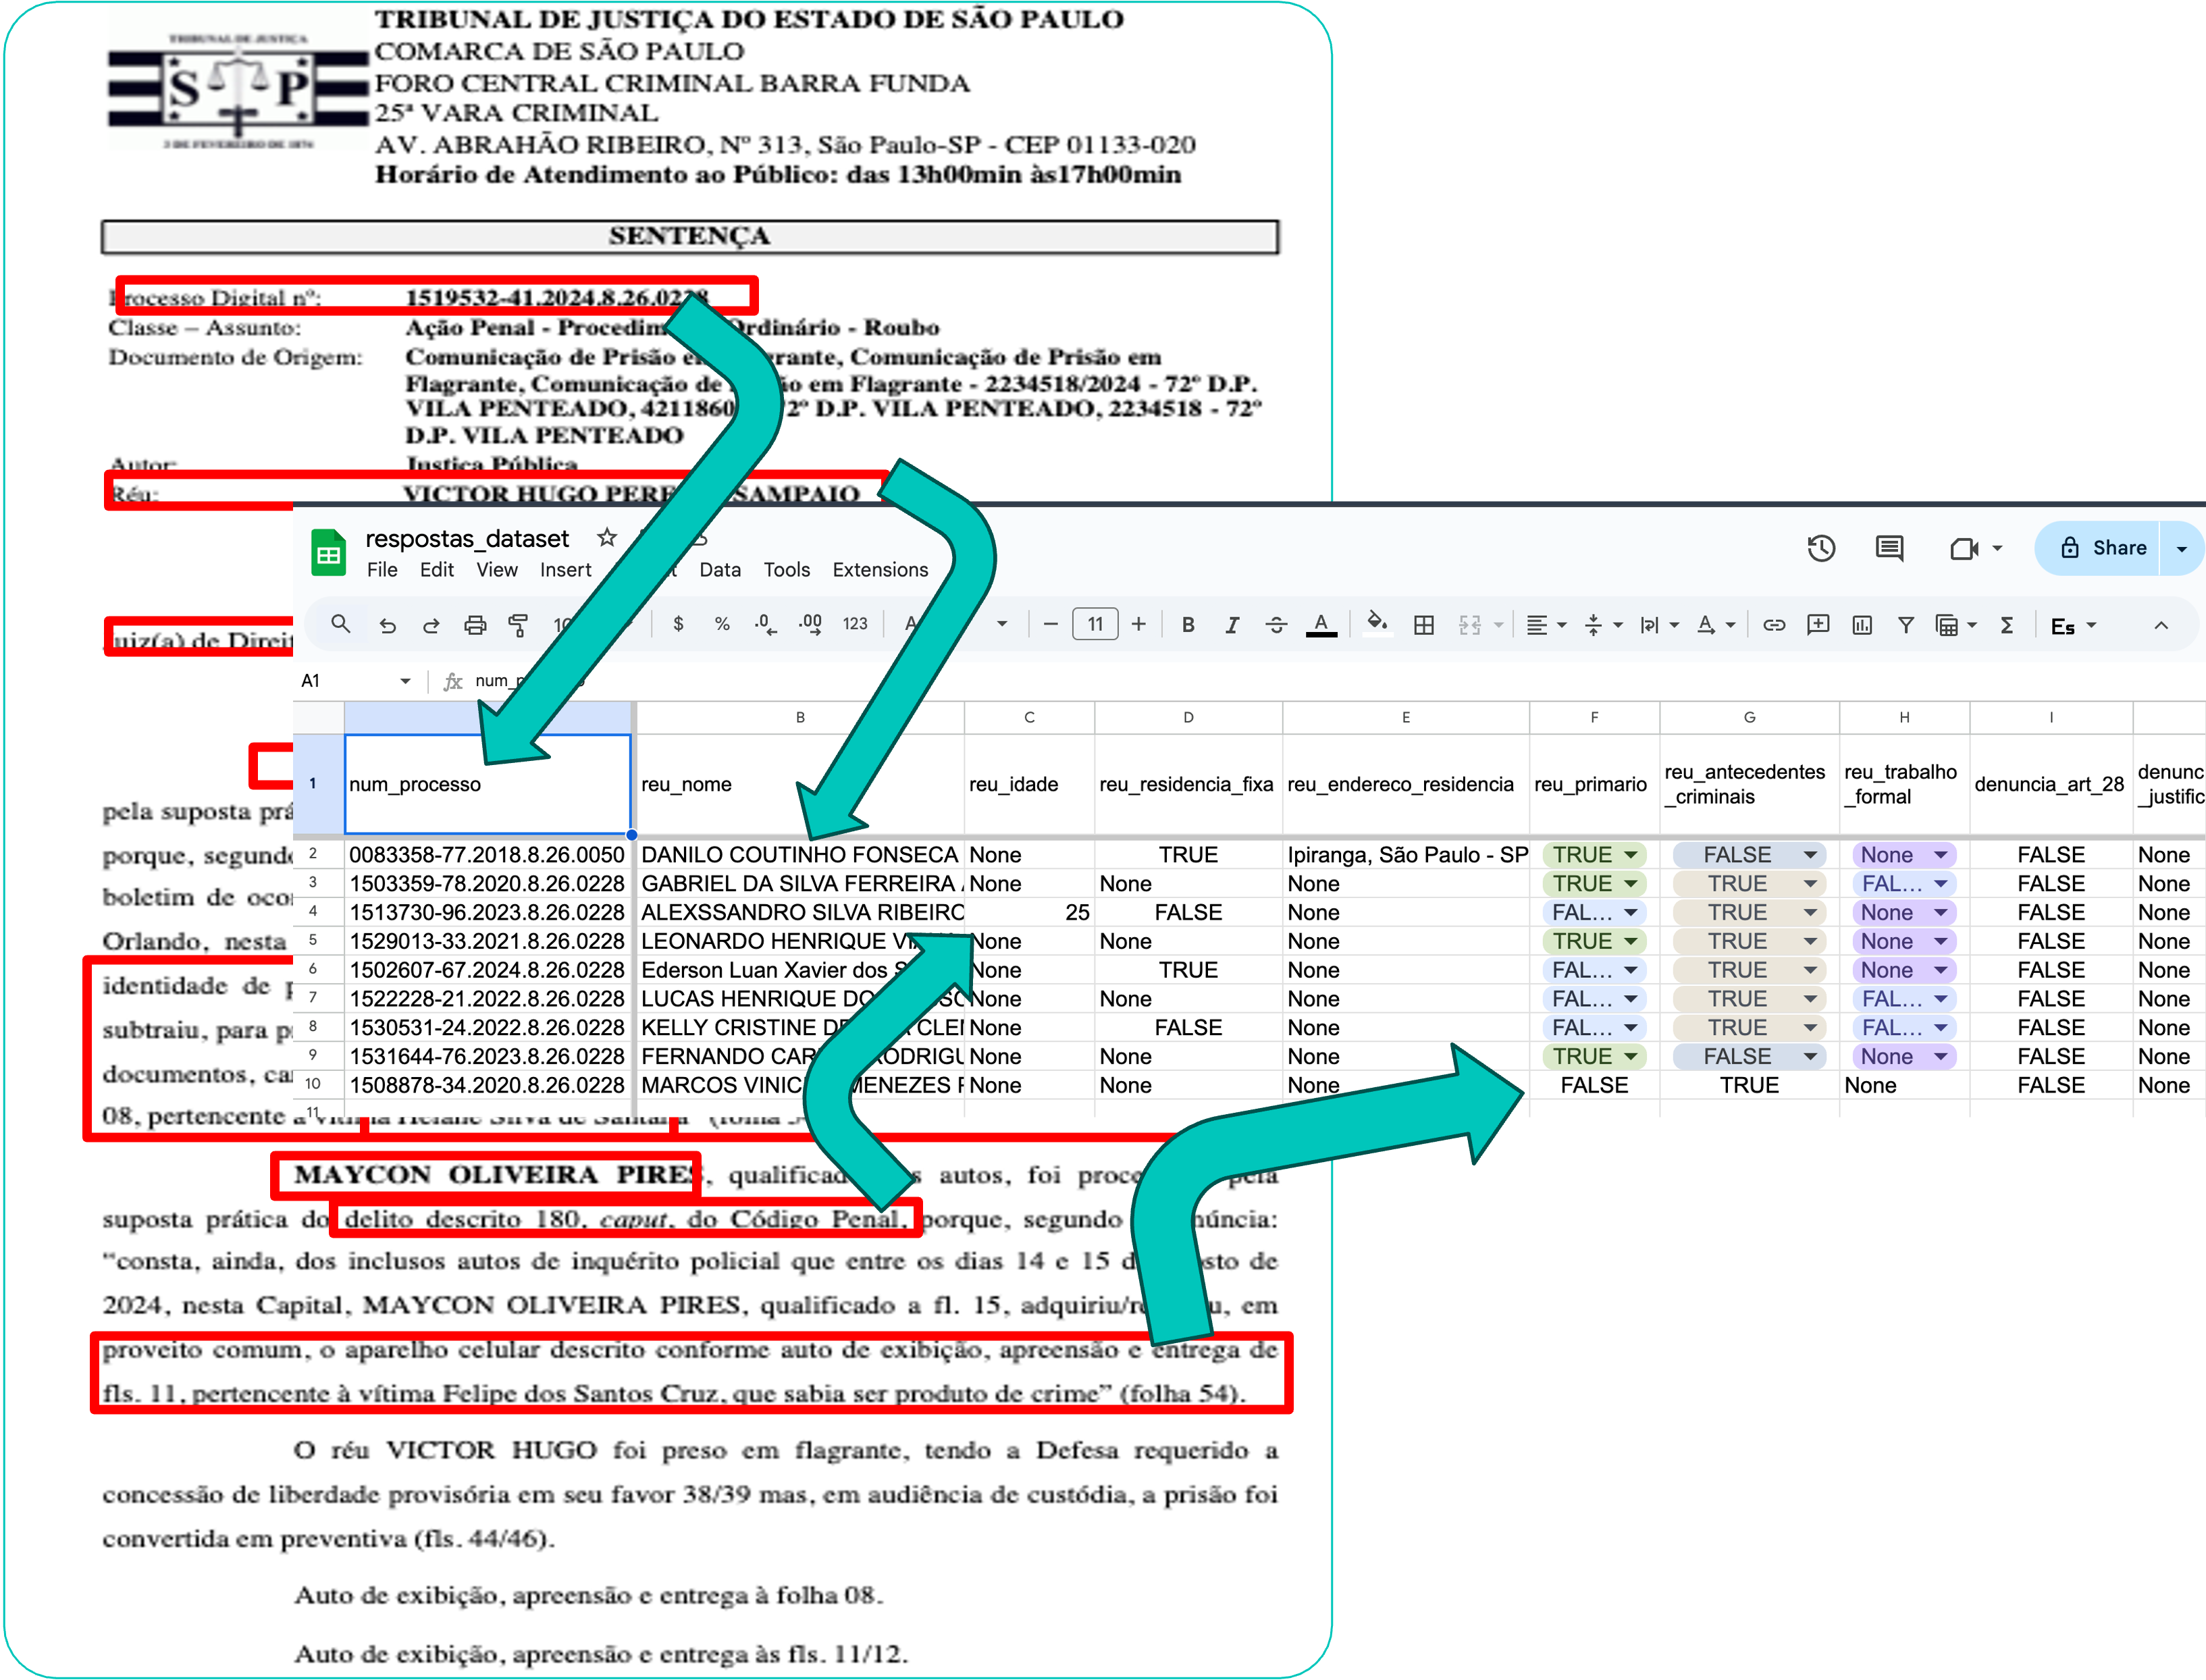
\includegraphics[width=5.20833in,height=\textheight,keepaspectratio]{images/schema-extraction.png}

}

\caption{\label{fig-schema-extraction}Illustration of the extraction of
information from a judicial decision. Multiple tasks depend on
understanding the text and following rules}

\end{figure}%

After the processes to gather and clean the data discussed before, the
steps were the following: 1) build a prompt and data schema, 2) pipeline
to run commercial models; 3) parsing algorithm, 4) evaluation algorithm;
5) pipeline to test open-source models and 6) pipeline to fine-tune
models.

Within this framework, choosing the more suitable LLMs for the task
would be possible. As discussed further, 12 models were tested with the
test dataset (containing 39 judicial sentences), and five were
fine-tuned.

All scripts were written in Python and R (in this case, the
visualizations and some data collection, as described in the
Section~\ref{sec-datasets}).

Regarding hardware, this research relied on Google Colab Pro (A100 GPU),
Kaggle (T4 GPU), and the Hertie School's GPU Server\footnote{\url{https://hertie-data-science.gitbook.io/hertie-school-gpu/extras/gpu-server-specs}}
(4x Nvidia A100\footnote{Despite some throttling issues caused by the
  high number of simultaneous users and the absence of a job management
  system, this research would not have been possible without the use of
  the GPU server. Thank you to the Data Science Lab for their support!}).
All the relevant experiment runnings were monitored using Weights and
Bias API (\citeproc{ref-biewald_experiment_2020}{Biewald, 2020}).

\subsection{Prompt and data schema}\label{prompt-and-data-schema}

Since the chosen models worked based on instructions, carefully
explaining the extraction task would be necessary. So, a comprehensive
prompt was written, explaining the general task, its subtasks, and how
each column should be filled out.

The prompt, written in Portuguese, explained the model its role, that it
would receive a judicial decision (``sentença'') related to criminal
cases in Brazil---specifically, drug trafficking. It also provided some
context about the general structure of the document (e.g., the head,
report, legal reasoning, dispositive part) and how to fill out each of
the columns.

The steps to answering the questions were carefully explained (such as
reading the whole document, using \emph{None} when something is not
mentioned, and interpreting the boolean columns in the whole document
context). Also, the prompt details how the answers should be, i.e., the
amount of a given drug should be a numerical answer in grams, the place
of detention should be picked among several options, and so on.

Specific instructions were provided regarding the output. Since the data
could not vary in its format---otherwise, it would not be possible to
transform it into a structured data frame---the model received specific
instructions to provide the answer in a valid JSON format, following a
given data schema.

\subsection{Pipeline to run commercial
models}\label{pipeline-to-run-commercial-models}

Although the scope of this research is to understand and asses if and
how open-source models would extract information, it was important to
establish a benchmark. OpenAI models were chosen since they represent
state of the art in many evaluations and are the most widespread
platform\footnote{\url{https://techcrunch.com/2025/04/01/chatgpt-isnt-the-only-chatbot-thats-gaining-users/?utm_source=chatgpt.com}}
\footnote{Also, there was the availability of using OpenAI platform
  through Hertie School's Data Science Lab account.}.

To access the models in OpenAI's platform, one must use an API. This API
offered the option to generate the outputs in batch mode, where the
whole test dataset was sent with the prompts in an asynchronous mode.
Batching allows for a 50\% reduction in costs and the receipt of data in
a single file containing all the responses generated.

To run each desired model, a batch was prepared, and the model and the
parameters were chosen. The file was uploaded, a batch generation was
started, and the results were downloaded back when ready. Regarding the
parameters, all OpenAI models were run with temperature at 0 level,
specifying the max tokens to be generated in 1.000, except with the
reasoning models without this option.

\subsection{Parsing algorithm}\label{parsing-algorithm}

The model's output will only be helpful if coerced into a tabular format
structured in a dataset object. If the model yields an answer in an
unstructured format, it cannot be evaluated or used in further
analysis---even if this answer is perfectly correct regarding its
content. For instance, by taking the example below in
Table~\ref{tbl-good-json-output}, we can see the correct values in the
desired JSON format.

\begin{table}

\centering{

\centering\begingroup\fontsize{9}{11}\selectfont

\begin{tabular}{>{\raggedright\arraybackslash}p{47em}}
\toprule
Correct JSON Output\\
\midrule
\{
 "processo": "0000922-86.2017.8.26.0635",
 "juiz": "Dr(a). Paula Marie Konno",
 "cocaina\_g": 42.4,
 "sentenca": "Procedente",
 "tot\_pen": "05a 500d"
\cellcolor{gray!10}{\}}\\
\bottomrule
\end{tabular}
\endgroup{}

}

\caption{\label{tbl-good-json-output}Example of correct output
(simplified version).}

\end{table}%

The following examples include several materially correct outputs but in
the wrong format. As we can see, we would have problems parsing them in
a structured data frame.

\begingroup\fontsize{9}{11}\selectfont

\begin{longtable}{>{\raggedright\arraybackslash}p{27em}>{\raggedright\arraybackslash}p{20em}}

\toprule
\multicolumn{2}{c}{Invalid Formats for Outputs} \\
\cmidrule(l{3pt}r{3pt}){1-2}
Example (invalid format) & Why is this invalid?\\
\midrule
\endfirsthead
\multicolumn{2}{@{}l}{\textit{(continued)}}\\
\toprule
Example (invalid format) & Why is this invalid?\\
\midrule
\endhead

\endfoot
\bottomrule
\endlastfoot
\cellcolor{gray!10}{The defendant was guilty. Judge Paula Marie Konno sentenced based on case 0000922-86.2017.8.26.0635. The total penalty was 05 years and 500 days-fine. 42.4 grams of cocaine were found.} & \cellcolor{gray!10}{Free-form narrative; does not follow a structured or machine-readable format.}\\
{}["0000922-86.2017.8.26.0635", "Paula Marie Konno", "42.4", "Procedente", "05a 500d"] & List without field identifiers; lacks explicit mapping to `processo`, `juiz`, `cocaina-g`, `sentenca`, and `tot-pen`.\\
\cellcolor{gray!10}{0000922-86.2017.8.26.0635, Paula Marie Konno, 42.4, Procedente, 05a 500d} & \cellcolor{gray!10}{CSV format without headers; field meanings are ambiguous and unsuitable for structured processing.}\\
\textbackslash{}\{'proc': '0000922-86.2017.8.26.0635', 'judge': 'Konno', 'cocaine': '42.4g', 'ruling': 'yes', 'pen': '5a500d'\textbackslash{}\} & Non-standard field names and mixed language; incorrect field types (e.g., cocaine as string with units).\\
\cellcolor{gray!10}{Processo ID: \textbackslash{}\#0000922-86-2017-8-26-0635 | J: P. M. Konno | Droga: Cocaína | Qtde: 42.4 | Resultado: sim | Pena: 5a + 500d} & \cellcolor{gray!10}{Custom syntax not aligned with standard field names (`processo`, `juiz`, `cocaina-g`, etc.); difficult to parse programmatically.}\\*


\caption{\label{tbl-bad-json-output}Examples of semantically correct but
structurally invalid outputs extracted from legal sentences.}

\tabularnewline
\end{longtable}

\endgroup{}

OpenAI (and other commercial models) offers a feature called JSON mode,
where it is possible to make sure that the answer will match the valid
schema offered. The open-source models, however, do not have this
feature out of the box. In the initial tests, giving only the models the
proper instructions and schema was insufficient.

The solution to this challenge was using PyDantic\footnote{Colvin et al.
  (\citeproc{ref-colvin_pydantic_2025}{2025})} and LangChain\footnote{Chase
  (\citeproc{ref-chase_langchain_2022}{2022})} libraries. The first
allows the generation of a class with the valid object and its
respective data types. The second offers a parsing structure to
constrain the result into a valid schema when possible. Naturally, when
the response is too different from the expected result, the answer will
be considered invalid in the evaluation phase.

\subsection{Evaluation algorithm: Accuracy}\label{sec-accuracy}

Evaluating is a key aspect of this research since it is relevant to
understand whether and how much the answers are correct. Establishing a
coherent strategy to evaluate the distinct models is also relevant.

The choice to use accuracy as the ideal metric is because the goal is to
understand how close the answers are to the ground truth, as used in
other papers such as
(\citeproc{ref-dominguez-olmedo_lawma_2024}{Dominguez-Olmedo et al.,
2024}; \citeproc{ref-junior_juru_2024}{Junior et al., 2024}). While
there are some sub-tasks, such as classifying the outcome of a decision
or comparing numeric answers, we would require a variety of metrics,
such as F1 score or mean squared error. These metrics must be uniformly
transformed into a single value to evaluate each model's performance.
However, this approach would significantly compromise interpretability
without providing clear benefits in understanding the overall
performance.

\begin{figure}[H]

\centering{

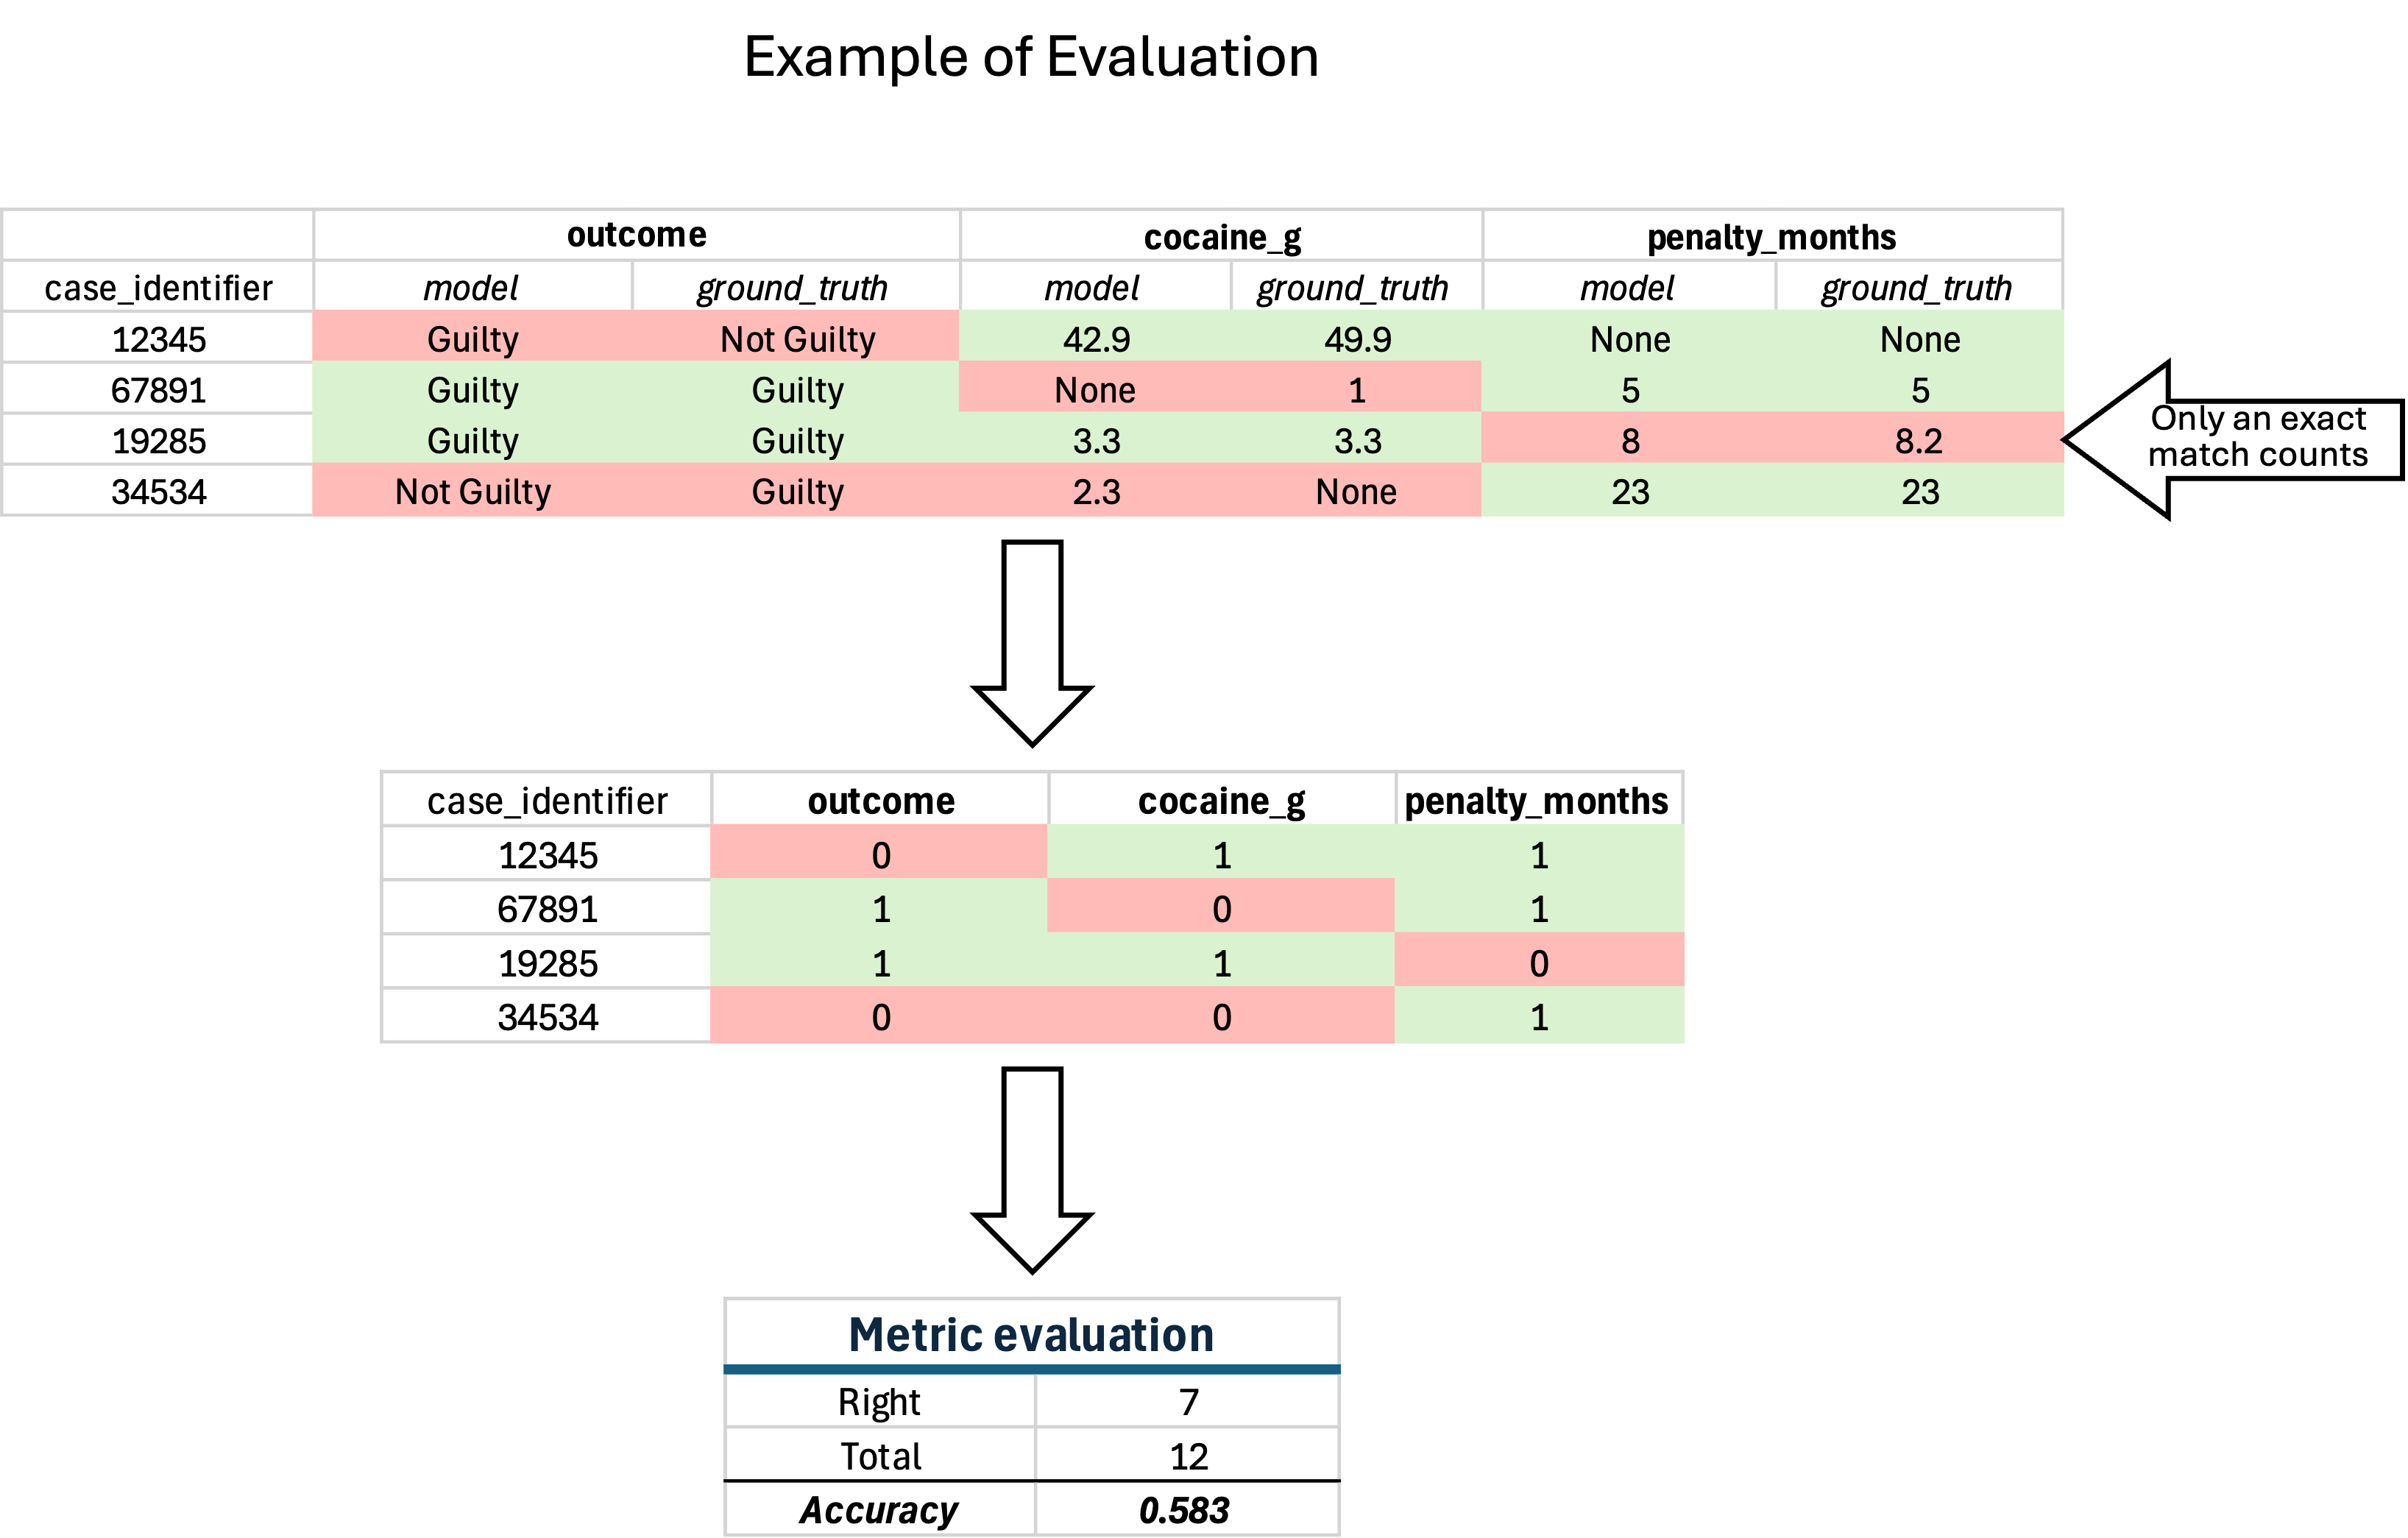
\includegraphics[width=5.20833in,height=\textheight,keepaspectratio]{images/example_eval.png}

}

\caption{\label{fig-example-eval}Example of the evaluation process}

\end{figure}%

The first step is to parse the results from the generated responses and
transform them into a data frame (called ``responses dataset'') with the
lawsuit number (column \textbf{processo}) as its unique
identifier\footnote{The Brazilian National Council of Justice (CNJ)
  regulates that this should be a preformatted and unique identifier for
  each lawsuit in the country.}. Notably, when a response is invalid,
the algorithm generates a row with only the ID filled out, leaving the
remaining columns empty.

Then, we have different evaluation functions according to the respective
data type (numeric, categorical, boolean, or open textual fields). The
different data types change the pre-processing step, but, in the end,
the model's response is compared with the ground truth
answer.\footnote{The functions were split also due to an attempt to
  establish different tolerance thresholds. However, in this work, all
  limits were stuck to zero, meaning there was no tolerance. The
  accuracy scores obtained might be slightly higher if one increases the
  level of tolerable differences.}

From this comparison, we will have a matrix with all answers and a value
of 0 if they do not match or 1 if they are right. Then, the sum of
correct answers will be divided by the total answers expected to assess
the accuracy. The accuracy was calculated using scikit-learn's function
\texttt{metrics.accuracy\_score}, which uses the following
formula\footnote{\url{https://scikit-learn.org/stable/modules/model_evaluation.html\#accuracy-score}}:

\begin{equation}\phantomsection\label{eq-accuracy}{
\texttt{accuracy}(y, \hat{y}) = \frac{1}{n_\text{samples}} \sum_{i=0}^{n_\text{samples}-1} 1(\hat{y}_i = y_i) 
}\end{equation}

According to Equation~\ref{eq-accuracy}, each model would achieve a
value between 0 and 1 according to its capabilities to generate correct
answers. This strategy also allows us to evaluate the accuracy in
specific columns, groups of columns, and other combinations, as needed.

\subsection{Pipeline to run open-source
models}\label{pipeline-to-run-open-source-models}

\subsubsection{Challenges and
strategies}\label{challenges-and-strategies}

A pipeline is needed to run and evaluate the results of the open-source
models (Section~\ref{sec-models}). Their reliability in terms of privacy
comes with the cost of setting them up, which brings some challenges
regarding the necessary computational resources, the size of the inputs
versus the window of context, and the output format.

One relevant challenge was the size of context windows. It is important
to consider that judicial sentences might be lengthy documents. In this
case, they were close primarily to 8k to 12k tokens (plus the prompt,
which has about 4k more), but it is also possible that they are way
bigger than that. Many models, as Table~\ref{tbl-metadata} shows, have
context windows way smaller than that.

Some techniques, such as Yarn (\citeproc{ref-peng_yarn_2023}{Peng et
al., 2023}) and RoPE scaling Tan
(\citeproc{ref-tan_extending_2024}{2024}), were first attempted to
enlarge those models' context windows artificially. However, they would
demand a heavy processing time, which is outside the scope of this
research, and, therefore, were discarded.

On the other hand, strategies such as chunking\footnote{\url{https://www.ibm.com/think/tutorials/chunking-strategies-for-rag-with-langchain-watsonx-ai}}
or Retrieval Augmented Generation (RAG)
(\citeproc{ref-lewis_retrieval-augmented_2021}{Lewis et al., 2021}) were
also attempted, with no good results. Besides their complexity, the
model would be unable to fully understand the document as a whole.
Although theoretically, it could fail in tasks such as evaluating
whether there are inconsistencies in the police officer's account since
it requires a complete understanding of the context.

The solution was to discard models such as LoLA, TucanoBR, Sabiá and
Lawma in favor of more general-use models with larger context windows.
Although the last three models were fine-tuned using our training
dataset, they could not produce the desired output. It does not mean
that these models are inferior to the others; instead, they were not
designed to meet this specific use case and, therefore, are unsuitable
for this specific task.

\subsubsection{Running open-source
models}\label{running-open-source-models}

After addressing the challenges, the open-source models were run and
evaluated using pipelines based on the HuggingFace Python framework
(\citeproc{ref-wolf_transformers_2020}{Wolf et al., 2020}). All
executions had the temperature set to 0 to avoid hallucinations as much
as possible, and the \emph{max\_tokens} value was set to 1.000.

Each model received batches containing the prompt and each of the
documents in the test dataset (Section~\ref{sec-datasets}). The results
were saved into individual \texttt{.json} files in the respective folder
and evaluated according to the parsing and evaluation strategies
(Section~\ref{sec-models}).

This same pipeline was used to run the open-source fine-tuned models, so
there was a reliable comparison with them before and after the process.

\subsection{Fine-tuning models}\label{fine-tuning-models}

The decision to fine-tune open-source models was due to the possibility
of `teaching' the general-use model how it should perform in a specific
task (\citeproc{ref-dominguez-olmedo_lawma_2024}{Dominguez-Olmedo et
al., 2024}; \citeproc{ref-junior_juru_2024}{Junior et al., 2024}). After
picking a model that was trained in billions of tokens, often in a
self-supervised way, the whole idea is to adjust some of their layers to
be able to reproduce the method of extracting information, using
transfer learning (\citeproc{ref-vajjala_practical_2020}{Vajjala et al.,
2020})

\subsubsection{Fine-tune OpenAI's
models}\label{fine-tune-openais-models}

In the case of OpenAI's models, the training pipeline was generated
using the API and run on their servers\footnote{\url{https://platform.openai.com/docs/guides/fine-tuning}}.

Also, the validation dataset was provided so the API could avoid
overfitting and optimize the parameters by itself. The model was trained
with auto-selection of parameters, which resulted in 3 epochs, a
learning rate multiplier of 1.80, and a batch size of 1.

The decision was to fine-tune only the GPT 4o-mini, not only because it
was the recommended option by OpenAI, but also because of the
costs\footnote{\url{https://openai.com/api/pricing/}}: the price of
using 4o-mini was 8.3x lower than fine-tunning 4o.

\subsubsection{Fine-tune Open Source
Models}\label{fine-tune-open-source-models}

Similar challenges to those faced with local inference were faced here,
but since fine-tuning is an even more demanding process, other
frameworks were necessary to make it possible due to the processing
constraints.

To make it possible to fine-tune, we relied on the Unsloth
framework\footnote{Daniel Han \& team
  (\citeproc{ref-daniel_han_unsloth_2023}{2023})}. It provides a to load
models into 4-bit or 8-bit quantization (reducing their size at the
price of a minor reduction in their precision) and applying LoRA to
train only the small amount of layers possible, usually around 1\%.
Following suggestions, we applied a rank and alpha of 16 Raschka
(\citeproc{ref-raschka_build_2024}{2024}), which led to a tiny
percentage of parameters being re-calculated.

After several attempts and errors, we decided to fine-tune\footnote{During
  the first phase of testing the models Lawma, Tucano and Sabiá were
  also attempted but they were not able to yield valid results.} Llama
3.2 (3B) and Phi-4. Although we had tried many other models (like those
from the Gemma3 family), they were not possible to fine-tune due to a
lack of memory and/or incompatibility with the current version of
libraries in the hardware.

\section{Results}\label{sec-results}

\subsection{Baseline performance}\label{baseline-performance}

To answer the research question (Section~\ref{sec-research_question}),
we need to understand how commercial and open-source models perform in a
zero-shot setting and the impact of fine-tuning on their performance.

After roughly 20 experiments\footnote{Ignoring validation tests and
  experiences to overcome the limitations regarding context windows or
  out-of-memory problems.}, the metrics above regarding
accuracy\footnote{By accuracy, we consider the proportion of exact
  answers relative to the total answers. It is better explained in
  Section~\ref{sec-accuracy}} were gathered. Below, we can see the
performance of the base models before fine-tuning.

\begin{longtable}[t]{llllr}

\toprule
family & type & model & parameters & accuracy\\
\midrule
\cellcolor{gray!10}{Gemma} & \cellcolor{gray!10}{open-source} & \cellcolor{gray!10}{Gemma 3} & \cellcolor{gray!10}{27 B} & \cellcolor{gray!10}{0.820}\\
OpenAI & commercial & GPT 4o & unknown & 0.788\\
\cellcolor{gray!10}{OpenAI} & \cellcolor{gray!10}{commercial} & \cellcolor{gray!10}{o3-mini} & \cellcolor{gray!10}{unknown} & \cellcolor{gray!10}{0.764}\\
Gemma & open-source & Gemma 3 & 12 B & 0.763\\
\cellcolor{gray!10}{OpenAI} & \cellcolor{gray!10}{commercial} & \cellcolor{gray!10}{GPT 4.1} & \cellcolor{gray!10}{unknown} & \cellcolor{gray!10}{0.755}\\
\addlinespace
Phi & open-source & Phi 4 & 14 B & 0.747\\
\cellcolor{gray!10}{Llama} & \cellcolor{gray!10}{open-source} & \cellcolor{gray!10}{Llama 3.1} & \cellcolor{gray!10}{8 B} & \cellcolor{gray!10}{0.735}\\
OpenAI & commercial & GPT 4o-mini & unknown & 0.711\\
\cellcolor{gray!10}{OpenAI} & \cellcolor{gray!10}{commercial} & \cellcolor{gray!10}{GPT 4.1-mini} & \cellcolor{gray!10}{unknown} & \cellcolor{gray!10}{0.697}\\
OpenAI & commercial & GPT 4.1-nano & unknown & 0.659\\
\addlinespace
\cellcolor{gray!10}{Llama} & \cellcolor{gray!10}{open-source} & \cellcolor{gray!10}{Llama 3.2} & \cellcolor{gray!10}{3 B} & \cellcolor{gray!10}{0.542}\\
Gemma & open-source & Gemma 3 & 1 B & 0.000\\
\bottomrule


\caption{\label{tbl-accuracy-metadata}Accuracy of base models}

\tabularnewline
\end{longtable}

The model Gemma 3-1B achieved 0.0 accuracy due to its inability to yield
valid structured JSON output and because, in many cases, the answers
only repeated the schema's example. The same happened with Lawma 8B,
Sabiá 7B, and Tucano 2B4: even after fine-tuning under the Unsloth
framework that applied Rope-scaling to enlarge the context windows, this
step was not enough to allow those models to generate valid results for
this research.

The model that performed best in a zero-shot approach was the Gemma
3-27B parameters, which surprisingly also beat the benchmark commercial
models, even GPT-4o. Also, the Gemma 3 family likely yields accurate
results since the lighter version with the 12B parameter performed very
well and was better than the newly released GPT-4.1.

The model Phi-4 also performed very well, beating OpenAI's smaller
models. Regarding the Llama family, the 3.1 version performed better
than the 4o-mini and the smaller GPT 4.1-mini and GPT 4.1-nano. On the
other hand, Llama 3.2 had an inferior performance in this setting.

Trying to understand a more fine-grained analysis, breaking the results
by the kind of tasks was possible. The \emph{numeric} tasks are those
related to extracting and calculating the number of drugs or prison time
in months: those tasks involved not only recognizing the numbers
(entities) but also `calculating' the final value. The \emph{boolean}
tasks are generally in the realm of question answering in a
TRUE/FALSE/None style (for instance, if art. 33 was the basis of the
sentence or if there were confessions by the defendant). The
\emph{categorical} tasks are those closely related to classification
tasks, such as the case's outcome (conviction, acquittal, etc). In this
case, the \emph{open textual} tasks are more likely to be similar to
named entity recognition: the name of the Judge and the defendant.

Trying to achieve a more fine-grained analysis, we restructured the
evaluation to group tasks by their underlying type. The named entity
recognition tasks involve identifying and extracting specific spans from
the decision, such as the names of judges or defendants. The numeric
question answering tasks require not just identifying numerical
information, but also performing basic calculations, for example,
summing prison times expressed in months.

Binary classification tasks correspond to simple two-way decisions ---
for instance, whether a legal basis like Article 33 was invoked.
Meanwhile, yes/no question answering tasks allow for slightly more
nuance (yes, no, or unclear), such as determining if the defendant
confessed during proceedings. Multiclass classification tasks involve
selecting the appropriate label among several possible outcomes, such as
the final decision in the case (conviction, acquittal, plea, etc.).
Finally, open text normalization tasks deal with normalizing free-text
fields, ensuring, for example, that variations of party names are
consistently matched to canonical forms.

\begin{figure}[H]

\centering{

\includegraphics[width=1\linewidth,height=\textheight,keepaspectratio]{../../evaluate_results/task_accuracy_heatmap_granular_nlp.png}

}

\caption{\label{fig-model_accuracy_nlp_tasks}Tasks by accuracy}

\end{figure}%

Across nearly all models, open text normalization and named entity
recognition tasks showed strong performance, while binary
classification, yes/no question answering, and multiclass classification
tasks presented greater variability. Numeric question answering tasks
generally performed well, although they demanded more complex reasoning
compared to straightforward entity extraction.

\subsection{Fine-tuned results}\label{fine-tuned-results}

Those results suggested that continuing to work with open-source models
was a promising strategy. Fine-tuning was performed with the models
OpenAI 4o-mini (which is the recommended model by OpenAI), Llama 3.2
(3B), and Phi4. No resources were available to perform fine-tuning on
other models. Despite many attempts, some of them, mainly from the Gemma
family, lacked full Unsloth library support during the experiments.

We fine-tuned the three selected models using a relatively small dataset
of 186 cases, always setting the temperature to the lowest value
possible. The model was trained in up to 3 epochs in OpenAI and 10 in
the open-source pipeline. In OpenAI, they ran 1 case per batch, while in
the open-source flow, the batches were 4 cases per step, with early
stopping set to up to 5 evaluation steps.

\begin{figure}[H]

\centering{


\includegraphics[width=0.6\linewidth,height=\textheight,keepaspectratio]{../../evaluate_results/finetune_losses.png}

}

\caption{\label{fig-ft_loss_evolution}Evolution in loss during
fine-tuning}

\end{figure}%

As Figure~\ref{fig-ft_loss_evolution} shows, all models showed
improvements in the loss even with a small dataset and within not so
many epochs. The early stopping parameter in the open-source
models\footnote{OpenAI has no such an option.} made Llama 3.2 (3B) stop
around epoch 9.8 and the Phi-4 model around 7.02. In all cases, the
plots suggest there would be some room to stop even earlier to make the
process more efficient.

\begin{figure}[H]

\centering{

\pandocbounded{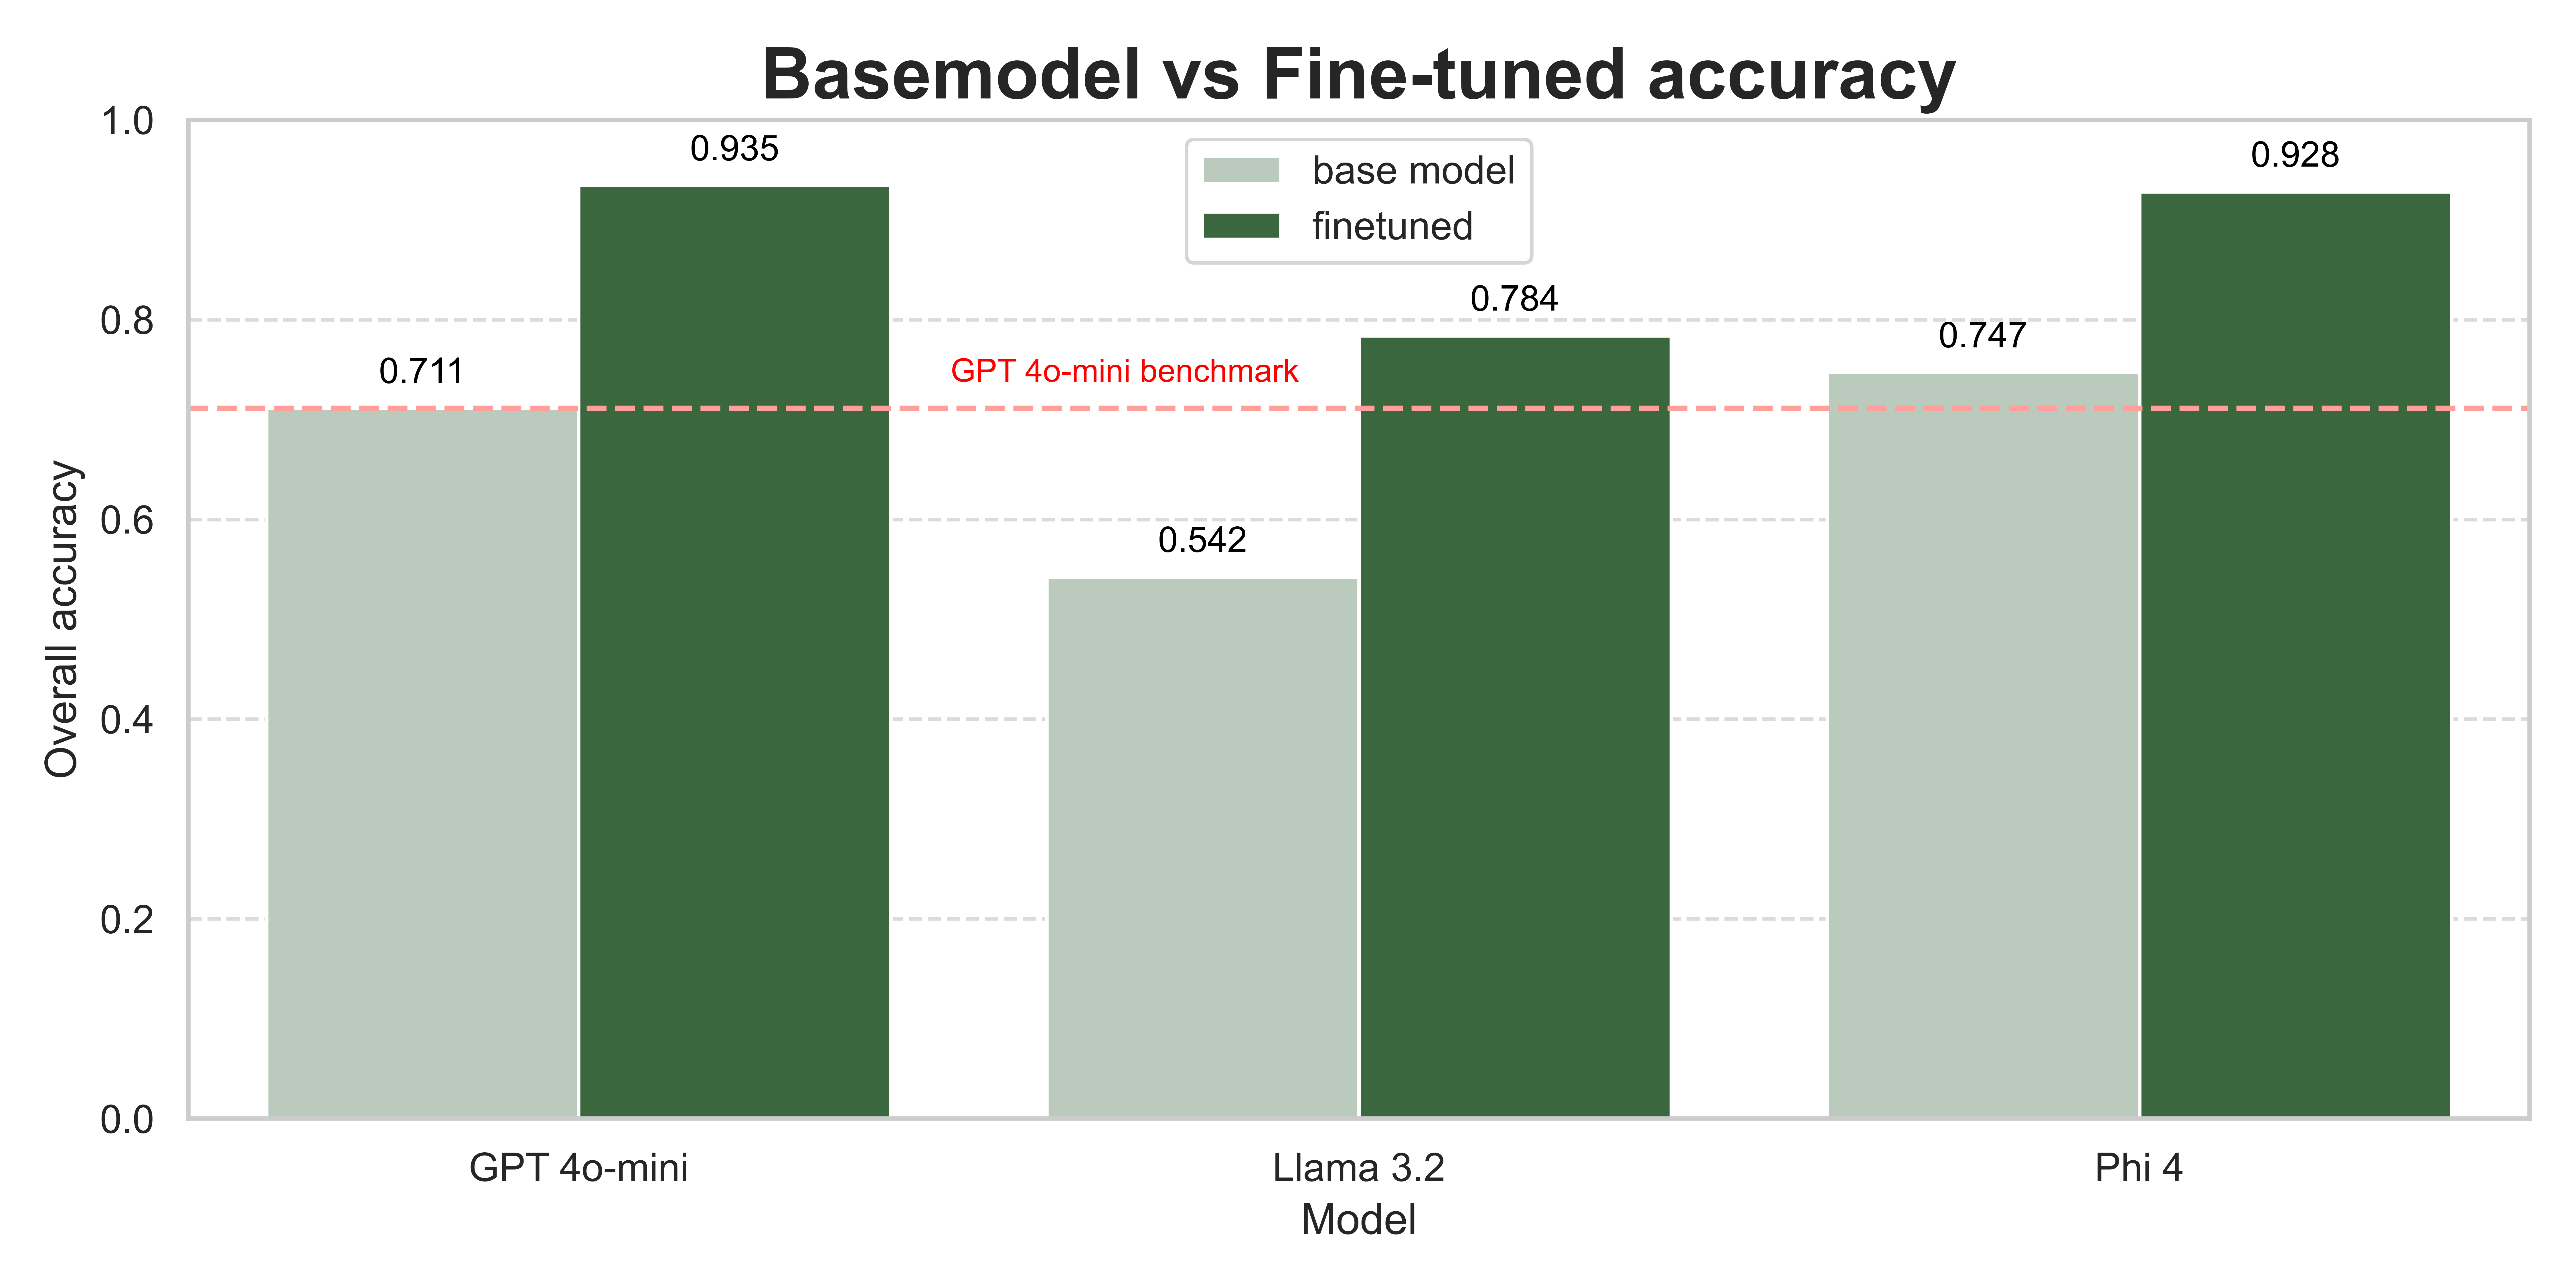
\includegraphics[keepaspectratio]{../../evaluate_results/base_vs_finetuned_accuracy.png}}

}

\caption{\label{fig-finetune}Models after fine-tuning}

\end{figure}%

As Figure~\ref{fig-finetune} showed, model Phi4 practicaly tied with GPT
4o-mini and the much smaller Llama 3.2 (3B) learned very easily, even
with both models being trained with the same 10 epochs.\footnote{With a
  richer dataset and/or more epochs, it would be possible to reach or
  even surpass GPT 4o-mini performance.}

\begin{table}

\begin{minipage}{0.50\linewidth}

\centering\begingroup\fontsize{8}{10}\selectfont

\resizebox{\ifdim\width>\linewidth\linewidth\else\width\fi}{!}{
\begin{tabular}{l|r|r|r}
\hline
metric & GPT 4o-mini & Llama 3.2 & Phi 4\\
\hline
\cellcolor{gray!10}{Δ accuracy} & \cellcolor{gray!10}{0.22} & \cellcolor{gray!10}{0.24} & \cellcolor{gray!10}{0.18}\\
\hline
Δ boolean & 0.29 & 0.20 & 0.21\\
\hline
\cellcolor{gray!10}{Δ categorical} & \cellcolor{gray!10}{-0.04} & \cellcolor{gray!10}{0.48} & \cellcolor{gray!10}{0.14}\\
\hline
Δ numeric & 0.11 & 0.28 & 0.09\\
\hline
\cellcolor{gray!10}{Δ open textual} & \cellcolor{gray!10}{0.01} & \cellcolor{gray!10}{0.21} & \cellcolor{gray!10}{0.08}\\
\hline
\end{tabular}}
\endgroup{}

\end{minipage}%
%
\begin{minipage}{0.50\linewidth}

\centering\begingroup\fontsize{8}{10}\selectfont

\resizebox{\ifdim\width>\linewidth\linewidth\else\width\fi}{!}{
\begin{tabular}{l|r|r|r}
\hline
metric & GPT 4o-mini & Llama 3.2 & Phi 4\\
\hline
\cellcolor{gray!10}{\% accuracy} & \cellcolor{gray!10}{31.37} & \cellcolor{gray!10}{44.57} & \cellcolor{gray!10}{24.16}\\
\hline
\% boolean & 43.56 & 34.54 & 28.63\\
\hline
\cellcolor{gray!10}{\% categorical} & \cellcolor{gray!10}{-4.46} & \cellcolor{gray!10}{145.31} & \cellcolor{gray!10}{17.76}\\
\hline
\% numeric & 14.44 & 62.15 & 11.17\\
\hline
\cellcolor{gray!10}{\% open textual} & \cellcolor{gray!10}{1.35} & \cellcolor{gray!10}{33.00} & \cellcolor{gray!10}{8.82}\\
\hline
\end{tabular}}
\endgroup{}

\end{minipage}%

\caption{\label{tbl-finetune-delta}Fine-tuned models: change in accuracy
(absolute value Δ and relative value \%)}

\end{table}%

As Table~\ref{tbl-finetune-delta} shows, Llama 3.2(3B) had the most
significant change in its performance, especially with the categorical
tasks. Specifically, with this task, we could see a performance
degradation of GPT 4o-mini. Phi4, \footnote{There is the
  \href{https://huggingface.co/microsoft/Phi-4-mini-instruct}{mini
  version of Phi-4}. However, it was impossible to run or fine-tune it
  with the current computational resources due to insufficient support
  from the Unsloth framework. Ref:
  \url{https://github.com/unslothai/unsloth/issues/2359}} though they
had the second-best performance, learned less than Llama, which suggests
a ceiling. Assuming that, in those architectures, the number of
parameters is the critical factor, fewer parameters than 14B and more
than 3B would be ideal.

\subsection{Inference performance}\label{inference-performance}

We conducted an inference on 454 decisions related to new drug
trafficking cases during the first quartile of 2024 and 2025. We
observed a significant difference in inference time by utilizing both
fine-tuned open-source models, Llama 3.2 (3B) and Phi-4.

The dataset encompasses 2,516,015 tokens\footnote{Considering the GPT-4
  tokenizer, as referenced in the Tiktoken library}. When accounting for
the prompt (approximately 3,000 tokens), the total consumption is
projected to reach 3,841,695 tokens. On average, we estimate this will
yield 252,029 output tokens with the max\_tokens parameter set to 1,000.

Regarding inference time, the Llama model required roughly 1 hour, 54
minutes for the entire batch, while Phi-4 took 4 hours, 7 minutes to
process the same batch, resulting in significantly longer individual
sample times. When considering costs, we can compare the three models by
examining the energy expenditures of the open-source models\footnote{Estimated
  energy costs: €0.2889 per KWh, EU average price in the first half of
  2024, according to
  \url{https://ec.europa.eu/eurostat/statistics-explained/index.php?title=Electricity_price_statistics\#Electricity_prices_for_household_consumers}}
and contrasting these with the inferred costs associated with OpenAI's
fine-tuned models\footnote{Assuming batch prices, which are the most
  economical, on April 26, 2025,
  \url{https://platform.openai.com/docs/pricing}. Assuming 1 USD = 0.88
  EUR}.

Below is a comparison detailing each model's performance in terms of
time, resource consumption, and associated costs to highlight the
differences.

\begin{longtable}[]{@{}llll@{}}

\toprule\noalign{}
Metric & Phi-4 & Llama 3.2-3B & GPT-4o-mini FT \\
\midrule\noalign{}
\endhead
\bottomrule\noalign{}
\endlastfoot
Total Time & 4:07:32 & 1:54:31 & unknown \\
Time/Sample (s) & 32.71 & 15.13 & unknown \\
Total Energy (kWh) & 1.596 & 0.814 & unknown \\
Total Cost (€) & 0.46 & 0.24 & 0.63 \\
Energy/Sample (Wh) & 3.52 & 1.79 & unknown \\


\caption{\label{tbl-inference-costs}Fine-tuned models: estimation on
inference time and costs}

\tabularnewline
\end{longtable}

\subsection{Limitations}\label{sec-limitations}

Since the test dataset is relatively small, with only 39 samples, the
generalization of the results should be seen with care, and one should
not expect the same high level of accuracy in other settings. Also, all
decisions in the dataset were from São Paulo's Court of Justice between
2017 and 2018 and only relative to drug possession cases: the size
constraints might limit the ability of the models to generalize in
judicial decisions from other areas of law or, even, from other Courts.

The size of the testing dataset also might have been insufficient to
assess if the fine-tuned models were overfitting to its context. In
addition, the years when the data was collected might influence the
final performance if applied to other periods since wording and
templates might change over the years. In this sense, new legislation
might affect how a giving decision is structured, thus impacting how the
model processes it.

Another important limitation is the prompt itself. It provides large
zero-shot instructions, and performance might be closely related to the
prompt style.

Since this method was crafted to extract information from many cases, it
is not ideal for extracting information from deeply complex and unique
decisions. Also, the window of context limits the method's applicability
to other contexts. Decisions with hundreds of pages and/or too much
complexity, common in Constitutional Courts, might not perform well in
similar settings.

Regarding evaluations, only using accuracy might have limited our
understanding of performance. Since we have not provided a balanced test
sample, it is possible that some higher scores were due to this fact.

Last, the models used carry different biases that were not tested in
this research. In addition, the annotation likely contains personal
perspectives and is not neutral (as it is impossible to be).

\section{Discussion}\label{sec-discussion}

\subsection{Key Findings}\label{sec-key-findinds}

We have found (Table~\ref{tbl-accuracy-metadata} and
Figure~\ref{fig-model_accuracy_nlp_tasks}) that commercial and
open-source models can enable jurimetric research. Many of them achieve
\textgreater{} 0.7 points of accuracy in a zero-shot setting, and GPT
4o-mini and Phi-4 achieve \textgreater{} 0.92 after fine-tuning. This
learning happens in all kinds of tasks (Table~\ref{tbl-finetune-delta}
and Table~\ref{tbl-finetune-delta}).

Even with a small dataset of 186 cases, applying LoRA and Quantization
through Unsloth (\citeproc{ref-daniel_han_unsloth_2023}{Daniel Han \&
team, 2023}) enabled the open-source models to learn the patterns quite
well, as Figure~\ref{fig-ft_loss_evolution} shows an important decrease
in the validation loss. Results suggest that even fewer epochs could
have been used.

When generating a dataset out of 454 new cases, fine-tuned versions of
GPT 4o-mini and Phi-4 -- that practically tied in their accuracy --, the
open-source model was 25\% cheaper than the commercial version
(Table~\ref{tbl-inference-costs}). Results show that open-source Phi-4
is cost-beneficial in similar settings. However, considering the
complexity of fine-tuning, it would be reasonable in many cases to pick
up the commercial models, especially if the price decreases in the
future. Although Phi-4 had an outstanding performance, it has a 16k
window context, which might be unfeasible in some contexts.

The fine-tuned version of LLama 3.2 (3B) was barely half the price and
inference time, at the cost of 20 percent points of accuracy. It would
be ideal to improve this model's accuracy through more complex training,
which may be achieved by tweaking the LoRA training factors or, ideally,
by a more comprehensive dataset. The efficient inference with far fewer
parameters suggests a promising performance.

Also, the Gemma3 family performed consistently well in few-shot
settings, . Although it has not been possible to fine-tune them to date,
they are promising architectures.

\subsection{Future Work}\label{sec-future-research}

There are important avenues to derive from this work. Having a larger
and more diverse high-quality dataset is key to the evolution of new
deployments. It would be ideal to have a few hundred judicial sentences
annotated in diverse fields from different Courts and even different
levels of jurisdiction.

Having more data would allow us to proceed with more robust tests of the
fine-tuned models and, especially, to break down the performance
measurement in different tasks. Also, it would allow us to tweak
hyperparameters and try to achieve improvements, especially regarding
Llama 3.2-like models.

We also suggest applying similar methods to train the Gemma3 family of
models once the technical challenges are overcome and trying other
families, such as Mistral, Anthropic, DeepSeek, and Qwen.

Another approach would be to generate results not as a whole but in
chunks of tasks, especially if there is a suggestion of at least a
proportional reduction in the inference time. However, this would not be
efficient with commercial models since the costs related to input tokens
would significantly increase.

Also, we do not know the prompt's importance in our experiments after
fine-tuning. More data would enable more testing in this aspect, leading
to an optimization of the generation prompt, making it easier to adapt
to other contexts.

Efficiency is another essential future path of work. Trying techniques
to prune models and distill their content would lead to lighter and more
efficient models. If models such as Tucano or Sabiá have larger context
windows optimized for instruction tuning, they might also be tested.
Also, as Figure~\ref{fig-finetune} suggests, some tests could be
conducted to make fine-tuning more efficient;
Table~\ref{tbl-finetune-delta} indicates that experiments with models
having 4B to 10B parameters could achieve an optimal efficiency.

Once we have a larger and more diverse dataset, it would not be a bad
idea to try to obtain a more flexible model that could generalize to
other legal contexts. This would allow researchers to spend less time
adapting existing models rather than just prompt engineering, which
tends to be faster and easier.

Although the results are specific to the Brazilian context, similar
approaches might be attempted in other jurisdictions and even with
different languages as long as the base models have idiomatic support
and there is enough training data in the legal task.

\subsection{Policy implications}\label{policy-implications}

It was clear the role that high-quality annotated data plays and the
potential that fine-tuning an LLM could have to accelerate empirical
legal research, easing the execution of data-driven research.

Our work's approach would allow the design of new research and the
update of other work that, due to the time-lapse, might not be as
informative as before. For instance, the models trained here would be
relevant to replicating Lacerda e Silva
(\citeproc{ref-lacerda_e_silva_punindo_2021}{2021}) work in recent
years, especially after the Brazilian Supreme Court decided on drug
decriminalization\footnote{https://www.conectas.org/en/noticias/nine-years-into-the-case-the-brazilian-federal-supreme-court-stf-decriminalizes-possession-of-marijuana-for-personal-use/}.

Regular analyses of topics such as civil compensations, labor claim
awards, consumer law, and others would also benefit legal practitioners
and public officials, enabling the identification of latent trends. A
rising success rate in a particular area could signal a forthcoming
surge in cases, as it would create incentives for litigants.
Anticipating such developments would be particularly important for the
administration of justice, especially regarding workforce allocation.

Legal firms, prosecutors, public defenders, and public attorneys might
apply a jurimetric approach to evaluate their own success rates,
understand which legal arguments are more relevant to their (in)success,
etc.

In academia, it would allow for a more comprehensive analysis of cases,
allowing researchers to have bigger samples, freeing them from the
intensive labor of annotating data, and allowing them to devote more
time to the substantive analysis itself.

\section{Conclusion}\label{sec-conclusion}

The results discussed above showed that, yes, open-source LLMs could
accurately extract information from judicial sentences and performed at
least as well as commercial models when fine-tuned and even beat them in
some zero-shot settings.

As Dominguez-Olmedo et al.
(\citeproc{ref-dominguez-olmedo_lawma_2024}{2024}) suggested, ``the
power of specialization'' is real: By using about two hundred
high-quality documents, we were able to increase the performance by
about 20 p.p Figure~\ref{fig-finetune}. Compared to commercial models,
the fine-tuned versions were also cheaper
Table~\ref{tbl-inference-costs}.

Besides the possibility of deploying open-source LLMs (specially
fine-tuned), the use of commercial models should not be excluded,
especially when there's no computational power and no privacy data
involved. In other words, there is a trade-off between commercial and
open-source models that would balance according to the task context.

The LLM field has been rapidly evolving in the last few years, as we can
see from Table~\ref{tbl-metadata}: almost all of the models used in this
research were released after May 2024. Libraries such as Unsloth and
Transformers allow easy deployment of open-source models, and they offer
promising perspectives regarding efficiency.

We are finally mature enough to adopt a more data-driven approach to
legal studies and promote more empirical research in this field.

\section{Policy Recommendations}\label{sec-policy-recommendations}

In order for this work to benefit the community most, we provide a few
recommendations aimed at strengthening data-driven empirical legal
research.

\textbf{Academia}: Disclose data from empirical legal research as much
as possible, as it would be a valuable resource for further fine-tuning
models. Obtaining data from past work and ensuring that the new research
data is available would accelerate the generation of new datasets,
benefiting the whole community. For instance, IPEA released the data
from Instituto de Pesquisa Econômica Aplicada (Ipea) \& Brasil.
Ministério da Justiça e Segurança Pública
(\citeproc{ref-instituto_de_pesquisa_economica_aplicada_ipea_perfil_2023}{2023}),
which would provide a larger and more diverse dataset.

\textbf{Judiciary branch}: Ensure data and lawsuit documents are
available digitally for research while maintaining high privacy
standards. Even if anonymized, keeping the data open in robust systems
such as DataJud\footnote{\url{https://www.cnj.jus.br/sistemas/datajud/}}
and the TJ-SP Judicial Decisions Database\footnote{\url{https://esaj.tjsp.jus.br/cjpg/}}
would ease access to legal documents and allow further research.

\textbf{Law schools}: Adapt the Law curriculum so scholars are data
literate. Future professionals should be aware of technology but
especially empowered by the new tools that artificial intelligence and
data science can already provide them.

\textbf{Think tanks and research networks}: Invest in jurimetric
research, gathering legal professionals and data scientists to
strengthen methodology and empirical evidence as much as possible.

\textbf{Open-source community}: Keep offering high-quality frameworks
such as Torch, HuggingFace, and Unsloth. The deployment of new LLMs
would be ideal if they maintained larger context windows (at least 20k
tokens) and efficient inference.

\textbf{Brazilian Ministry of Science and Technology}: Offer
computational resources, with a robust GPU framework, to accelerate
empirical research in the country and to reduce the dependency on
external cloud providers.

Lastly, it remains clear that domain knowledge was a key factor in
success throughout the process. So, it is strongly advisable not to
shorten or cut research job positions in favor of ``substituting'' human
labor with a large language model. To believe that it could be simply
`automated' would be a big mistake since the conception and design need
a deep understanding of the legal field under analysis. Not having
enough human oversight during operation would lead to mistakes being
massively replicated and more subtle biases not being identified.

This work shows that models should not replace legal work and that legal
experts should not be reduced to data annotations but rather be involved
in the whole process.

\newpage{}

\section{References}\label{sec-references}

\phantomsection\label{refs}
\begin{CSLReferences}{1}{0}
\bibitem[\citeproctext]{ref-abdin_phi-4_2024}
Abdin, M., Aneja, J., Behl, H., Bubeck, S., Eldan, R., Gunasekar, S.,
Harrison, M., Hewett, R. J., Javaheripi, M., Kauffmann, P., Lee, J. R.,
Lee, Y. T., Li, Y., Liu, W., Mendes, C. C. T., Nguyen, A., Price, E.,
Rosa, G. de, Saarikivi, O., \ldots{} Zhang, Y. (2024). \emph{Phi-4
{Technical} {Report}}. arXiv.
\url{https://doi.org/10.48550/arXiv.2412.08905}

\bibitem[\citeproctext]{ref-almeida_sabia-2_2024}
Almeida, T. S., Abonizio, H., Nogueira, R., \& Pires, R. (2024).
\emph{Sabiá-2: {A} {New} {Generation} of {Portuguese} {Large} {Language}
{Models}}. arXiv. \url{https://doi.org/10.48550/arXiv.2403.09887}

\bibitem[\citeproctext]{ref-alves_da_silva_aspectos_2022}
Alves da Silva, P. E. (2022). Aspectos metodológicos da pesquisa
empírica em {Direito} com processos judiciais físicos e eletrônicos. In
\emph{Estudos empíricos em processo e organização judiciária}. Expert.

\bibitem[\citeproctext]{ref-de_andrade_utilizacao_2018}
Andrade, M. D. de. (2018). A utilização do sistema {R}-studio e da
jurimetria como ferramentas complementares à pesquisa jurídica / {The}
use of the {R}-studio system and jurimetrics as complementary tools for
the legal research. \emph{REVISTA QUAESTIO IURIS}, \emph{11}(2),
680--692. \url{https://doi.org/10.12957/rqi.2018.29221}

\bibitem[\citeproctext]{ref-associacao_brasileira_de_jurimetria_avaliacao_2019}
Associação Brasileira de Jurimetria. (2019). \emph{Avaliação do
{Impacto} de {Critérios} {Objetivos} na {Distinção} {Entre} {Posse} para
{Uso} e {Posse} para {Tráfico}: {Um} estudo {Jurimétrico}}. Associação
Brasileira de Jurimetria.
\url{https://abj.org.br/pdf/20190402_abj_criterios_objetivos.pdf}

\bibitem[\citeproctext]{ref-benatti_gender_2024}
Benatti, R., Severi, F., Avila, S., \& Colombini, E. L. (2024). Gender
{Bias} {Detection} in {Court} {Decisions}: {A} {Brazilian} {Case}
{Study}. \emph{Proceedings of the 2024 {ACM} {Conference} on {Fairness},
{Accountability}, and {Transparency}}, 746--763.
\url{https://doi.org/10.1145/3630106.3658937}

\bibitem[\citeproctext]{ref-biewald_experiment_2020}
Biewald, L. (2020). \emph{Experiment {Tracking} with {Weights} and
{Biases}}. \url{https://www.wandb.com/}

\bibitem[\citeproctext]{ref-cabrera_de_bonito_pesquisa_2025}
Cabrera De Bonito, B., Veloso De Castro, C., \& Korasaki, V. (2025).
{PESQUISA} {QUANTITATIVA} {NO} {DIREITO}: {UMA} {REVISÃO}
{BIBLIOGRÁFICA}. \emph{Revista de Estudos Empíricos Em Direito},
\emph{11}. \url{https://doi.org/10.19092/reed.v11.830}

\bibitem[\citeproctext]{ref-chase_langchain_2022}
Chase, H. (2022). \emph{{LangChain}}.
\url{https://github.com/langchain-ai/langchain}

\bibitem[\citeproctext]{ref-colvin_pydantic_2025}
Colvin, S., Jolibois, E., Ramezani, H., Garcia Badaracco, A., Dorsey,
T., Montague, D., Matveenko, S., Trylesinski, M., Runkle, S., Hewitt,
D., Hall, A., \& Plot, V. (2025). \emph{Pydantic}.
\url{https://github.com/pydantic/pydantic}

\bibitem[\citeproctext]{ref-correa_tucano_2024}
Corrêa, N. K., Sen, A., Falk, S., \& Fatimah, S. (2024). \emph{Tucano:
{Advancing} {Neural} {Text} {Generation} for {Portuguese}}. arXiv.
\url{https://doi.org/10.48550/arXiv.2411.07854}

\bibitem[\citeproctext]{ref-costa_eficacia_2011}
Costa, S. H. da, Silva, P. E. A. da, Sabino, M. A. da C., Fernandes, D.
C. M., \& Lusvarghi, L. A. dos S. (2011). \emph{A eficácia do sistema
jurídico de prevenção e combate à improbidade administrativa}
{[}Publicação de relatório de pesquisa{]}. Secretaria de Assuntos
Legislativos do Ministério da Justiça.
\url{https://web.archive.org/web/20211004195943/http://pensando.mj.gov.br/wp-content/uploads/2015/07/34Pensando_Direito1.pdf}

\bibitem[\citeproctext]{ref-daniel_han_unsloth_2023}
Daniel Han, M. H., \& team, U. (2023). \emph{Unsloth}.
\url{http://github.com/unslothai/unsloth}

\bibitem[\citeproctext]{ref-dominguez-olmedo_lawma_2024}
Dominguez-Olmedo, R., Nanda, V., Abebe, R., Bechtold, S., Engel, C.,
Frankenreiter, J., Gummadi, K., Hardt, M., \& Livermore, M. (2024).
\emph{Lawma: {The} {Power} of {Specialization} for {Legal} {Tasks}}.
arXiv. \url{http://arxiv.org/abs/2407.16615}

\bibitem[\citeproctext]{ref-dragoni_combining_2016}
Dragoni, M., Villata, S., Rizzi, W., \& Governatori, G. (2016,
December). Combining {NLP} {Approaches} for {Rule} {Extraction} from
{Legal} {Documents}. \emph{1st {Workshop} on {MIning} and {REasoning}
with {Legal} Texts ({MIREL} 2016)}.
\url{https://hal.science/hal-01572443}

\bibitem[\citeproctext]{ref-filho_coleta_2020}
Filho, J. de J., \& Trecenti, J. (2020). \emph{Coleta e organização de
dados do {Tribunal} de {Justiça} de {São} {Paulo}}.
\url{https://jjesufilho.github.io/tjsp/}

\bibitem[\citeproctext]{ref-instituto_de_pesquisa_economica_aplicada_ipea_perfil_2023}
Instituto de Pesquisa Econômica Aplicada (Ipea), \& Brasil. Ministério
da Justiça e Segurança Pública. (2023). \emph{Perfil do processado e
produção de provas nas ações criminais por tráfico de drogas : Relatório
analítico nacional dos {Tribunais} {Estaduais} de {Justiça} {Comum}}.
Instituto de Pesquisa Econômica Aplicada (Ipea).
\url{https://doi.org/10.38116/ri221151}

\bibitem[\citeproctext]{ref-junior_juru_2024}
Junior, R. M., Pires, R., Romero, R., \& Nogueira, R. (2024).
\emph{Juru: {Legal} {Brazilian} {Large} {Language} {Model} from
{Reputable} {Sources}}. arXiv.
\url{https://doi.org/10.48550/arXiv.2403.18140}

\bibitem[\citeproctext]{ref-lacerda_e_silva_punindo_2021}
Lacerda e Silva, M. (2021). \emph{Punindo as diferenças: {Gênero}, raça
e geração no sentenciamento de tráfico de drogas na cidade de {São}
{Paulo}}. \url{http://repositorio.unb.br/handle/10482/41413}

\bibitem[\citeproctext]{ref-lewis_retrieval-augmented_2021}
Lewis, P., Perez, E., Piktus, A., Petroni, F., Karpukhin, V., Goyal, N.,
Küttler, H., Lewis, M., Yih, W., Rocktäschel, T., Riedel, S., \& Kiela,
D. (2021). \emph{Retrieval-{Augmented} {Generation} for
{Knowledge}-{Intensive} {NLP} {Tasks}}. arXiv.
\url{https://doi.org/10.48550/arXiv.2005.11401}

\bibitem[\citeproctext]{ref-loevinger_jurimetricsnext_1948}
Loevinger, L. (1948). Jurimetrics--{The} {Next} {Step} {Forward}.
\emph{Minn. L. Rev.}, \emph{33}, 455.

\bibitem[\citeproctext]{ref-niklaus_multilegalpile_2023}
Niklaus, J., Matoshi, V., Sturmer, M., Chalkidis, I., \& Ho, D. E.
(2023). \emph{{MultiLegalPile}: {A} {689GB} {Multilingual} {Legal}
{Corpus}}. \url{https://doi.org/10.48550/arXiv.2306.02069}

\bibitem[\citeproctext]{ref-openai_gpt-4_2024}
OpenAI, Achiam, J., Adler, S., Agarwal, S., Ahmad, L., Akkaya, I.,
Aleman, F. L., Almeida, D., Altenschmidt, J., Altman, S., Anadkat, S.,
Avila, R., Babuschkin, I., Balaji, S., Balcom, V., Baltescu, P., Bao,
H., Bavarian, M., Belgum, J., \ldots{} Zoph, B. (2024). \emph{{GPT}-4
{Technical} {Report}}. \url{https://arxiv.org/abs/2303.08774}

\bibitem[\citeproctext]{ref-peng_yarn_2023}
Peng, B., Quesnelle, J., Fan, H., \& Shippole, E. (2023). \emph{{YaRN}:
{Efficient} {Context} {Window} {Extension} of {Large} {Language}
{Models}}. arXiv. \url{https://doi.org/10.48550/arXiv.2309.00071}

\bibitem[\citeproctext]{ref-pires_sabia_2023}
Pires, R., Abonizio, H., Almeida, T. S., \& Nogueira, R. (2023).
\emph{Sabiá: {Portuguese} {Large} {Language} {Models}} (Vol. 14197, pp.
226--240). \url{https://doi.org/10.1007/978-3-031-45392-2_15}

\bibitem[\citeproctext]{ref-raschka_build_2024}
Raschka, S. (2024). \emph{Build a {Large} {Language} {Model} (from
{Scratch})}. Manning Publications Co. LLC.
\url{http://ebookcentral.proquest.com/lib/hertie-school/detail.action?docID=31657639}

\bibitem[\citeproctext]{ref-ribeiro_jurimetria_2022}
Ribeiro, E. M. S., Rodello, I. A., \& Morilas, L. R. (2022). Jurimetria:
As possibilidades e os desafios de um modelo para a análise empírica dos
processos e dos atores processuais. In G. M. Gonçalves, R. C. V. Maia,
I. M. Rocha, \& G. P. Teodoro (Eds.), \emph{Estudos empíricos em
processo e organização judiciária}. Editora Expert.
\url{https://experteditora.com.br/wp-content/uploads/2022/02/Estudos-empiricos-em-processo-e-organizacao-judiciaria.pdf}

\bibitem[\citeproctext]{ref-su_roformer_2023}
Su, J., Lu, Y., Pan, S., Murtadha, A., Wen, B., \& Liu, Y. (2023).
\emph{{RoFormer}: {Enhanced} {Transformer} with {Rotary} {Position}
{Embedding}}. arXiv. \url{https://doi.org/10.48550/arXiv.2104.09864}

\bibitem[\citeproctext]{ref-tan_extending_2024}
Tan, L. (2024). Extending context length with {Hugging} {Face}'s
transformers. In \emph{Medium}.
\url{https://medium.com/@leannetan/extending-context-length-with-hugging-faces-transformers-6b04db05b39a}

\bibitem[\citeproctext]{ref-team_gemma_2025}
Team, G., Kamath, A., Ferret, J., Pathak, S., Vieillard, N., Merhej, R.,
Perrin, S., Matejovicova, T., Ramé, A., Rivière, M., Rouillard, L.,
Mesnard, T., Cideron, G., Grill, J., Ramos, S., Yvinec, E., Casbon, M.,
Pot, E., Penchev, I., \ldots{} Hussenot, L. (2025). \emph{Gemma 3
{Technical} {Report}}. arXiv.
\url{https://doi.org/10.48550/arXiv.2503.19786}

\bibitem[\citeproctext]{ref-vajjala_practical_2020}
Vajjala, S., Majumder, B., Gupta, A., \& Surana, H. (2020).
\emph{Practical {Natural} {Language} {Processing}: {A} {Comprehensive}
{Guide} to {Building} {Real}-{World} {NLP} {Systems}}. "O'Reilly Media,
Inc.".

\bibitem[\citeproctext]{ref-wickham_r_2023}
Wickham, H., Çetinkaya-Rundel, M., \& Grolemund, G. (2023). \emph{R for
{Data} {Science}} (2nd ed.). O'Reilly Media.
\url{https://r4ds.hadley.nz/}

\bibitem[\citeproctext]{ref-wolf_transformers_2020}
Wolf, T., Debut, L., Sanh, V., Chaumond, J., Delangue, C., Moi, A.,
Cistac, P., Ma, C., Jernite, Y., Plu, J., Xu, C., Le Scao, T., Gugger,
S., Drame, M., Lhoest, Q., \& Rush, A. M. (2020). \emph{Transformers:
{State}-of-the-{Art} {Natural} {Language} {Processing}}. 38--45.
\url{https://www.aclweb.org/anthology/2020.emnlp-demos.6}

\bibitem[\citeproctext]{ref-zhang_dive_2023}
Zhang, A., Lipton, Z. C., Li, M., \& Smola, A. J. (2023). \emph{Dive
into {Deep} {Learning}}. arXiv.
\url{https://doi.org/10.48550/arXiv.2106.11342}

\end{CSLReferences}

\clearpage
\appendix

\section{Appendix - Plots and tables}\label{sec-plots-tables}

\begin{figure}[H]

\centering{

\includegraphics[width=1\linewidth,height=\textheight,keepaspectratio]{../../evaluate_results/per_task_accuracy_comparison.png}

}

\caption{\label{fig-accuracy-comparison}Accuracy comparison - Finetuned
models - Kind of datatype}

\end{figure}%

\begin{figure}[H]

\centering{


\includegraphics[width=1\linewidth,height=\textheight,keepaspectratio]{../../evaluate_results/task_accuracy_heatmap_granular_nlp_finetuned.png}

}

\caption{\label{fig-task-accuracy-heatmap}Task accuracy heatmap -
Fine-tuned models}

\end{figure}%

\begin{figure}[H]

\centering{

\includegraphics[width=1\linewidth,height=\textheight,keepaspectratio]{../../evaluate_results/radar_charts_per_experiment.png}

}

\caption{\label{fig-radar-charts}Radar charts comparing performance by
datatype}

\end{figure}%

\section{Appendix - Description of NLP Tasks}\label{sec-nlp-tasks}

\begingroup\fontsize{7}{9}\selectfont

\begin{longtable}[t]{>{\raggedright\arraybackslash}p{15em}>{\raggedright\arraybackslash}p{17em}>{\raggedright\arraybackslash}p{17em}}

\toprule
column & data\_type\_task & nlp\_task\\
\midrule
\cellcolor{gray!10}{maconha\_g} & \cellcolor{gray!10}{numeric} & \cellcolor{gray!10}{numeric\_qa}\\
cocaina\_g & numeric & numeric\_qa\\
\cellcolor{gray!10}{crack\_g} & \cellcolor{gray!10}{numeric} & \cellcolor{gray!10}{numeric\_qa}\\
ecstasy\_g & numeric & numeric\_qa\\
\cellcolor{gray!10}{lsd\_g} & \cellcolor{gray!10}{numeric} & \cellcolor{gray!10}{numeric\_qa}\\
\addlinespace
tot\_pen\_meses & numeric & numeric\_qa\\
\cellcolor{gray!10}{aval\_antecedentes} & \cellcolor{gray!10}{boolean} & \cellcolor{gray!10}{binary\_classification}\\
aval\_conduta & boolean & binary\_classification\\
\cellcolor{gray!10}{aval\_personalidade} & \cellcolor{gray!10}{boolean} & \cellcolor{gray!10}{binary\_classification}\\
aval\_natureza & boolean & binary\_classification\\
\addlinespace
\cellcolor{gray!10}{aval\_quantidade} & \cellcolor{gray!10}{boolean} & \cellcolor{gray!10}{binary\_classification}\\
aval\_variedade & boolean & binary\_classification\\
\cellcolor{gray!10}{aval\_circunstancias} & \cellcolor{gray!10}{boolean} & \cellcolor{gray!10}{binary\_classification}\\
aval\_consequencias & boolean & binary\_classification\\
\cellcolor{gray!10}{aval\_culpabilidade} & \cellcolor{gray!10}{boolean} & \cellcolor{gray!10}{binary\_classification}\\
\addlinespace
resultado\_art\_28 & boolean & binary\_classification\\
\cellcolor{gray!10}{resultado\_art\_33} & \cellcolor{gray!10}{boolean} & \cellcolor{gray!10}{binary\_classification}\\
resultado\_art\_34 & boolean & binary\_classification\\
\cellcolor{gray!10}{resultado\_art\_35} & \cellcolor{gray!10}{boolean} & \cellcolor{gray!10}{binary\_classification}\\
denuncia\_art\_33 & boolean & binary\_classification\\
\addlinespace
\cellcolor{gray!10}{denuncia\_art\_34} & \cellcolor{gray!10}{boolean} & \cellcolor{gray!10}{binary\_classification}\\
denuncia\_art\_35 & boolean & binary\_classification\\
\cellcolor{gray!10}{maconha} & \cellcolor{gray!10}{boolean} & \cellcolor{gray!10}{yesno\_qa}\\
maconha\_outras & boolean & yesno\_qa\\
\cellcolor{gray!10}{cocaina} & \cellcolor{gray!10}{boolean} & \cellcolor{gray!10}{yesno\_qa}\\
\addlinespace
crack & boolean & yesno\_qa\\
\cellcolor{gray!10}{ecstasy} & \cellcolor{gray!10}{boolean} & \cellcolor{gray!10}{yesno\_qa}\\
lsd & boolean & yesno\_qa\\
\cellcolor{gray!10}{outras\_drogas} & \cellcolor{gray!10}{boolean} & \cellcolor{gray!10}{yesno\_qa}\\
flag\_local\_de\_trafico & boolean & yesno\_qa\\
\addlinespace
\cellcolor{gray!10}{flag\_preso\_no\_momento\_da\_sentenca} & \cellcolor{gray!10}{boolean} & \cellcolor{gray!10}{yesno\_qa}\\
flag\_confissao\_informal & boolean & yesno\_qa\\
\cellcolor{gray!10}{flag\_confissao} & \cellcolor{gray!10}{boolean} & \cellcolor{gray!10}{yesno\_qa}\\
flag\_denuncia\_anonima & boolean & yesno\_qa\\
\cellcolor{gray!10}{flag\_denuncia} & \cellcolor{gray!10}{boolean} & \cellcolor{gray!10}{yesno\_qa}\\
\addlinespace
flag\_atitude\_suspeita & boolean & yesno\_qa\\
\cellcolor{gray!10}{flag\_divergencias\_nos\_relatos\_dos\_policiais} & \cellcolor{gray!10}{boolean} & \cellcolor{gray!10}{yesno\_qa}\\
flag\_investigacao & boolean & yesno\_qa\\
\cellcolor{gray!10}{flag\_interceptacao} & \cellcolor{gray!10}{boolean} & \cellcolor{gray!10}{yesno\_qa}\\
flag\_mandado & boolean & yesno\_qa\\
\addlinespace
\cellcolor{gray!10}{local} & \cellcolor{gray!10}{categorical} & \cellcolor{gray!10}{multiclass\_classification}\\
sentenca & categorical & multiclass\_classification\\
\cellcolor{gray!10}{juiz} & \cellcolor{gray!10}{open\_textual} & \cellcolor{gray!10}{open\_text\_normalization}\\
nome & open\_textual & open\_text\_normalization\\
\cellcolor{gray!10}{pena\_base} & \cellcolor{gray!10}{span} & \cellcolor{gray!10}{named\_entity\_recognition}\\
\addlinespace
tot\_pen & span & named\_entity\_recognition\\
\bottomrule


\caption{\label{tbl-nlp-task}Mapping of columns to traditional NLP
tasks}

\tabularnewline
\end{longtable}

\endgroup{}

\section{Appendix - Lacerda's Original Dataset
Description}\label{sec-lacerda-dataset}

\textbf{Variable type: character}

\begin{longtable}[]{@{}
  >{\raggedright\arraybackslash}p{(\linewidth - 14\tabcolsep) * \real{0.2658}}
  >{\raggedleft\arraybackslash}p{(\linewidth - 14\tabcolsep) * \real{0.1266}}
  >{\raggedleft\arraybackslash}p{(\linewidth - 14\tabcolsep) * \real{0.1772}}
  >{\raggedleft\arraybackslash}p{(\linewidth - 14\tabcolsep) * \real{0.0506}}
  >{\raggedleft\arraybackslash}p{(\linewidth - 14\tabcolsep) * \real{0.0506}}
  >{\raggedleft\arraybackslash}p{(\linewidth - 14\tabcolsep) * \real{0.0759}}
  >{\raggedleft\arraybackslash}p{(\linewidth - 14\tabcolsep) * \real{0.1139}}
  >{\raggedleft\arraybackslash}p{(\linewidth - 14\tabcolsep) * \real{0.1392}}@{}}

\toprule\noalign{}
\begin{minipage}[b]{\linewidth}\raggedright
skim\_variable
\end{minipage} & \begin{minipage}[b]{\linewidth}\raggedleft
n\_missing
\end{minipage} & \begin{minipage}[b]{\linewidth}\raggedleft
complete\_rate
\end{minipage} & \begin{minipage}[b]{\linewidth}\raggedleft
min
\end{minipage} & \begin{minipage}[b]{\linewidth}\raggedleft
max
\end{minipage} & \begin{minipage}[b]{\linewidth}\raggedleft
empty
\end{minipage} & \begin{minipage}[b]{\linewidth}\raggedleft
n\_unique
\end{minipage} & \begin{minipage}[b]{\linewidth}\raggedleft
whitespace
\end{minipage} \\
\midrule\noalign{}
\endhead
\bottomrule\noalign{}
\endlastfoot
Processo & 0 & 1 & 20 & 26 & 0 & 352 & 0 \\
DtDisp & 0 & 1 & 5 & 10 & 0 & 210 & 0 \\
Juiz & 0 & 1 & 13 & 49 & 0 & 79 & 0 \\
Vara & 0 & 1 & 16 & 17 & 0 & 32 & 0 \\
Nome & 0 & 1 & 11 & 39 & 0 & 419 & 0 \\
Local & 0 & 1 & 7 & 19 & 0 & 10 & 0 \\
Sexo & 0 & 1 & 8 & 9 & 0 & 2 & 0 \\
DN & 0 & 1 & 5 & 28 & 0 & 411 & 0 \\
Cutis & 0 & 1 & 5 & 7 & 0 & 5 & 0 \\
Cabelo & 0 & 1 & 4 & 16 & 0 & 8 & 0 \\
Objetos & 0 & 1 & 4 & 159 & 0 & 261 & 0 \\
Maconha & 0 & 1 & 1 & 41 & 0 & 255 & 0 \\
Cocaína & 0 & 1 & 1 & 38 & 0 & 274 & 0 \\
Crack & 1 & 1 & 1 & 40 & 0 & 138 & 0 \\
Ecstasy & 0 & 1 & 1 & 24 & 0 & 12 & 0 \\
LSD & 0 & 1 & 1 & 18 & 0 & 6 & 0 \\
Outras & 0 & 1 & 1 & 61 & 0 & 33 & 0 \\
DenDrog & 0 & 1 & 7 & 25 & 0 & 4 & 0 \\
DenOutros & 0 & 1 & 3 & 51 & 0 & 13 & 0 \\
Aspectos & 0 & 1 & 6 & 122 & 0 & 156 & 0 \\
Sentença & 0 & 1 & 10 & 23 & 0 & 5 & 0 \\
ResDrogas & 0 & 1 & 2 & 25 & 0 & 6 & 0 \\
ResOutros & 0 & 1 & 2 & 45 & 0 & 16 & 0 \\
AvalNegPB & 0 & 1 & 2 & 50 & 0 & 28 & 0 \\
PenaBase & 0 & 1 & 2 & 12 & 0 & 18 & 0 \\
Agravantes33 & 0 & 1 & 2 & 12 & 0 & 3 & 0 \\
Atenuantes33 & 0 & 1 & 2 & 21 & 0 & 5 & 0 \\
Aumento33 & 0 & 1 & 2 & 26 & 0 & 8 & 0 \\
§4º & 0 & 1 & 2 & 13 & 0 & 5 & 0 \\
Pena33 & 0 & 1 & 2 & 10 & 0 & 46 & 0 \\
PenaDrogas & 0 & 1 & 2 & 5 & 0 & 7 & 0 \\
PenaOutros & 0 & 1 & 2 & 9 & 0 & 15 & 0 \\
TotPen & 0 & 1 & 2 & 11 & 0 & 59 & 0 \\
Substituição da pena & 0 & 1 & 2 & 3 & 0 & 3 & 0 \\
Regime inicial & 0 & 1 & 2 & 10 & 0 & 4 & 0 \\


\caption{\label{tbl-lacerda}Lacerda's Original Dataset}

\tabularnewline
\end{longtable}

\newpage{}

\section{Appendix - Acknowledgments}\label{sec-thank-you}

\emph{Caminante, no hay camino, se hace camino al andar} (Antonio
Machado)\footnote{*``Traveller, there is no path; the path is made by
  walking.''}

This Master's Thesis would not be possible without the dataset carefully
annotated and generously provided by Marina Lacerda Silva, who dared to
do a jurimetric master's thesis a few years ago. I could only put
together this work under the supervision of Prof.~Lynn Kaack --- and,
also, thanks for her Deep Learning course --- and other brilliant
colleagues also under her supervision. There would not be possible to
conduct many experiments in this thesis without the support of Huy Dang
and the Hertie School Data Science Lab. I am also grateful for Maria
Utenthal's insights in the first conception of this research idea. Thank
you all!

Also, this work is part of a long path initiated way before me. A
special thank you to Prof.~Susana Henriques da Costa, who first
introduced me to the possibilities (and struggles) of legal empirical
research and got me excited about doing research. Another important
thank you to Prof.~Paulo Eduardo Alves da Silva, Prof.~José Jesus Filho,
and Prof.~Julio Tecenti for their contributions to the jurimetric field
in Brazil.

Although this thesis is only one more step on this \emph{camino} to a
master's degree in Data Science for Public Policy, it allows me to thank
those who helped me reach this point. A very heartfelt thank you to
Katia and Juares, my parents, who never hesitated to support me even
when they did not understand my choices. \emph{Muito obrigado!}

Thank you, Motriz, for the Vetor Brasil Scholarship and to Chancen Eg
for giving me the financial conditions to enroll in this program! This
research benefited largely from time spent with the Berkeley Equity and
Access in Algorithms, Mechanisms, and Optimization (BEAAMO) Summer
Fellowship Program. Thank you, Prof.~Rediet Abebe, and my colleagues
Mírian Silva, Rayssa Benatti, and Tainá Turella! It is also a good
opportunity to thank my colleagues from Jusbrasil (especially the
Analytics and the Legal Team) for having many chances to apply data
science to the legal context and have inspiring conversations every day.

Also, I would like to thank my colleagues from the MDS classes 2024 and
2025, the Latin-American Club (and the members of the `Latin Pomodoro'),
the Hertie School Digital Verification Corps, and many brilliant
colleagues whom I had the chance to share conversations and a good time
together in the Makerspace, the Library, and the cafeteria.

Since it's impossible to nominate them all, I will thank you with a deep
\emph{muito obrigado} my friends Henrique Motta, João Vítor Krieger,
Paulina Boechat, Renan Fernandes, and the whole Brazilian-Hertian
community! This journey in Berlin would not be possible without the
presence and support of Francisco Rios, Ana Barros, and the other
friends from Urso, who brought some rhythm to this journey.

Last but not least, I would like to thank many others who have supported
my journey and helped me abroad by being present during many of the
steps that I took here. Thank you, Vitor Moneo, Fernanda Horn, Orisha,
and Meirelles!

Having said that, a grateful thank you to any eventual reader! I hope
this work contributes to better legal research, improves our
institutions, and, thus, positively impacts people's lives.




\end{document}
